\section{Evaluation}
\label{sec:evaluation}

\subsection{Setup}

We have evaluated our implementation in an environment consisting on two
computers located in the same Gigabit Ethernet network.  We run the \broker,
\garbler and one Subscriber on the first computer, and all the Publishers in
the second computer.  We perform all the analysis on the performance of several
operations in the \broker and \garbler, which run together in a computer
running Arch Linux (kernel 4.8.17-grsec) with an Intel Core i7-6600U CPU with
16GB of RAM.  In order to isolate the performance influence of the \broker and
the \garbler, we have serialized the garbling and evaluation of the garbled
circuit operations (forbidding evaluation operations while the \garbler is
garbling), mimicking the situation in which the \broker and \garbler are run on
different servers.  We also forbid concurrent garbling operations and
concurrent evaluation operations to avoid high fluctuations in the measures.

Since the \broker and the \garbler are running on the same computer, we won't
observe the delay introduced by transferring the garbled circuit over a
physical network.  For this reason we obtain an estimation of the time required
to send the garbled circuit by simulating a transmission over a Gigabit
bandwidth network.  Since we know the size of the garbled circuit, we can
easily compute the time required to transfer it over a Gigabit connection and
add that delay to the measured time.

Our current implementation doesn't support the Private Set Intersection between
\broker and \garbler used to guarantee that the labels sent by the Publishers
are valid for the garbled circuit.  In order to evaluate this step of the
protocol we have run simulations of an implementation of the Private Set
Intersection based on Oblivious Transfer extension~\cite{Pinkas0Z14}, using the
number of labels corresponding to 32 bit values.

In all our measured times, sending includes the marshaling and unmarshaling of
the garbled circuit and associated data structures necessary for transmitting
it from the \garbler to the \broker via RPC.

\vspace{-10pt}
\subsection{Microbenchmarks}

\begin{figure*}[ht]
    \centering
    \begin{subfigure}[b]{0.32\textwidth}
        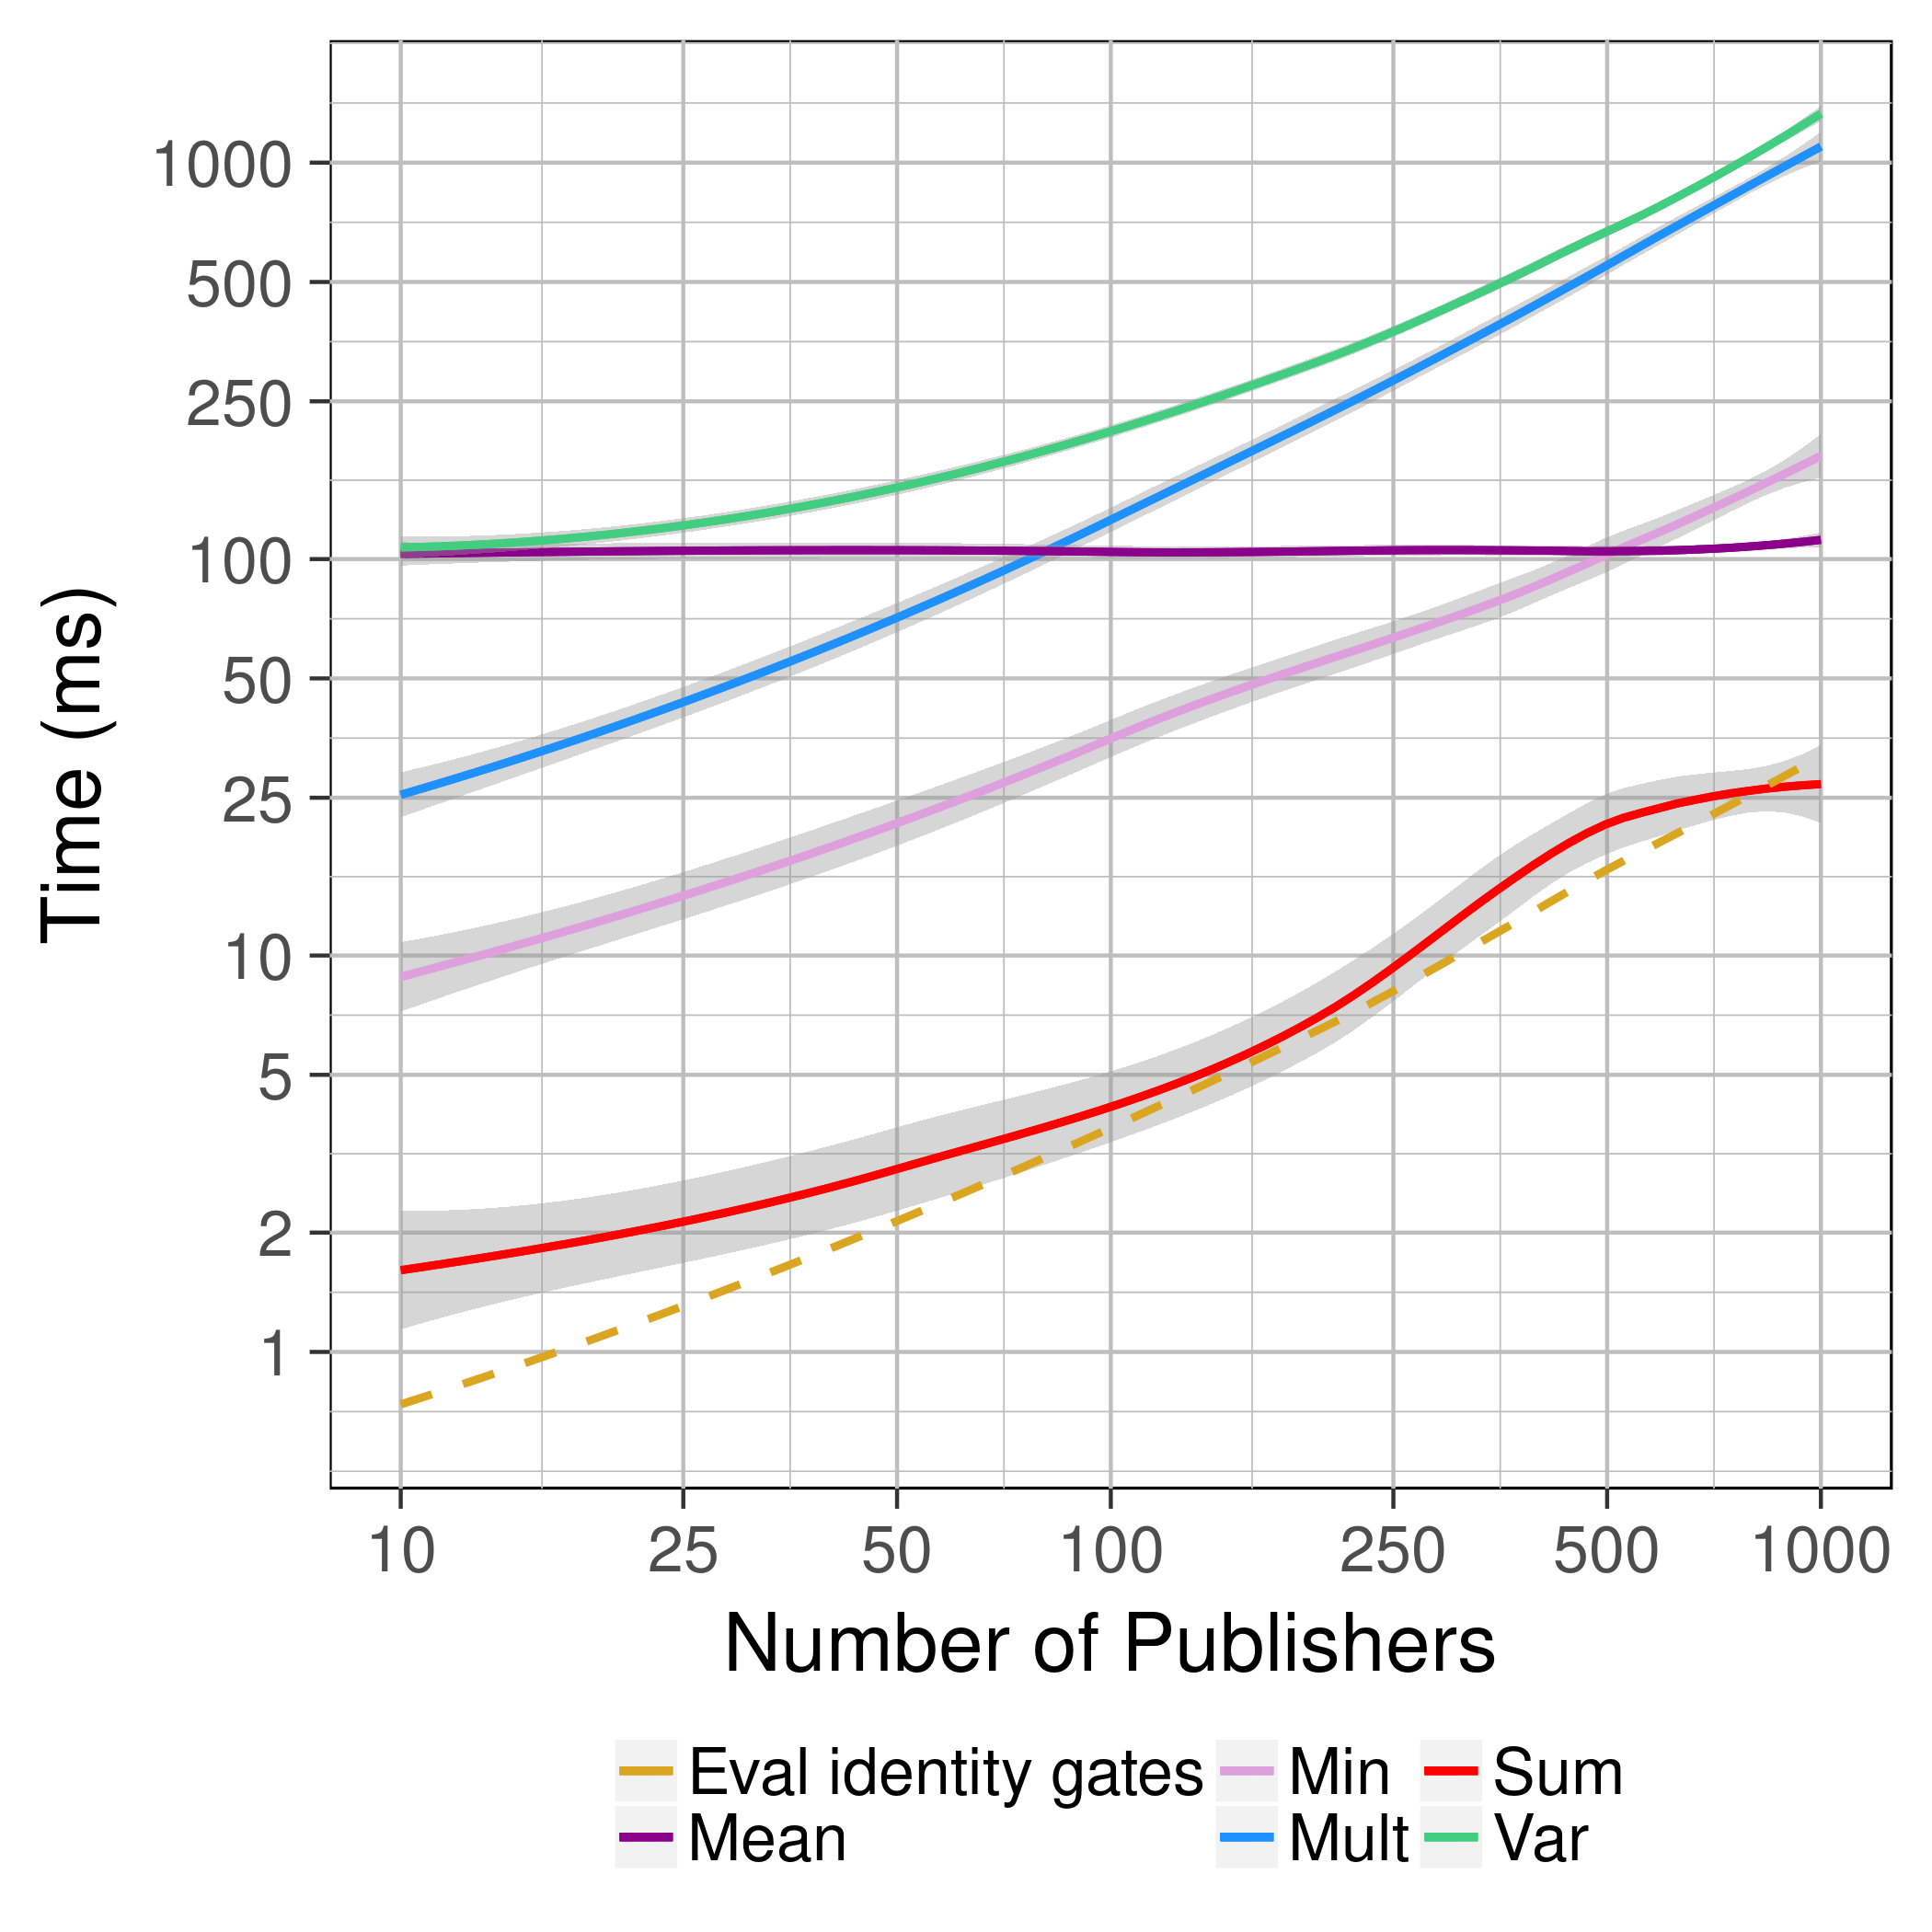
\includegraphics[width=\textwidth]{plots/garble_loglog.png}
        \caption{Garble}
        \label{fig:micro-garble-time}
    \end{subfigure}
    ~ %add desired spacing between images, e. g. ~, \quad, \qquad, \hfill etc.
    \begin{subfigure}[b]{0.32\textwidth}
        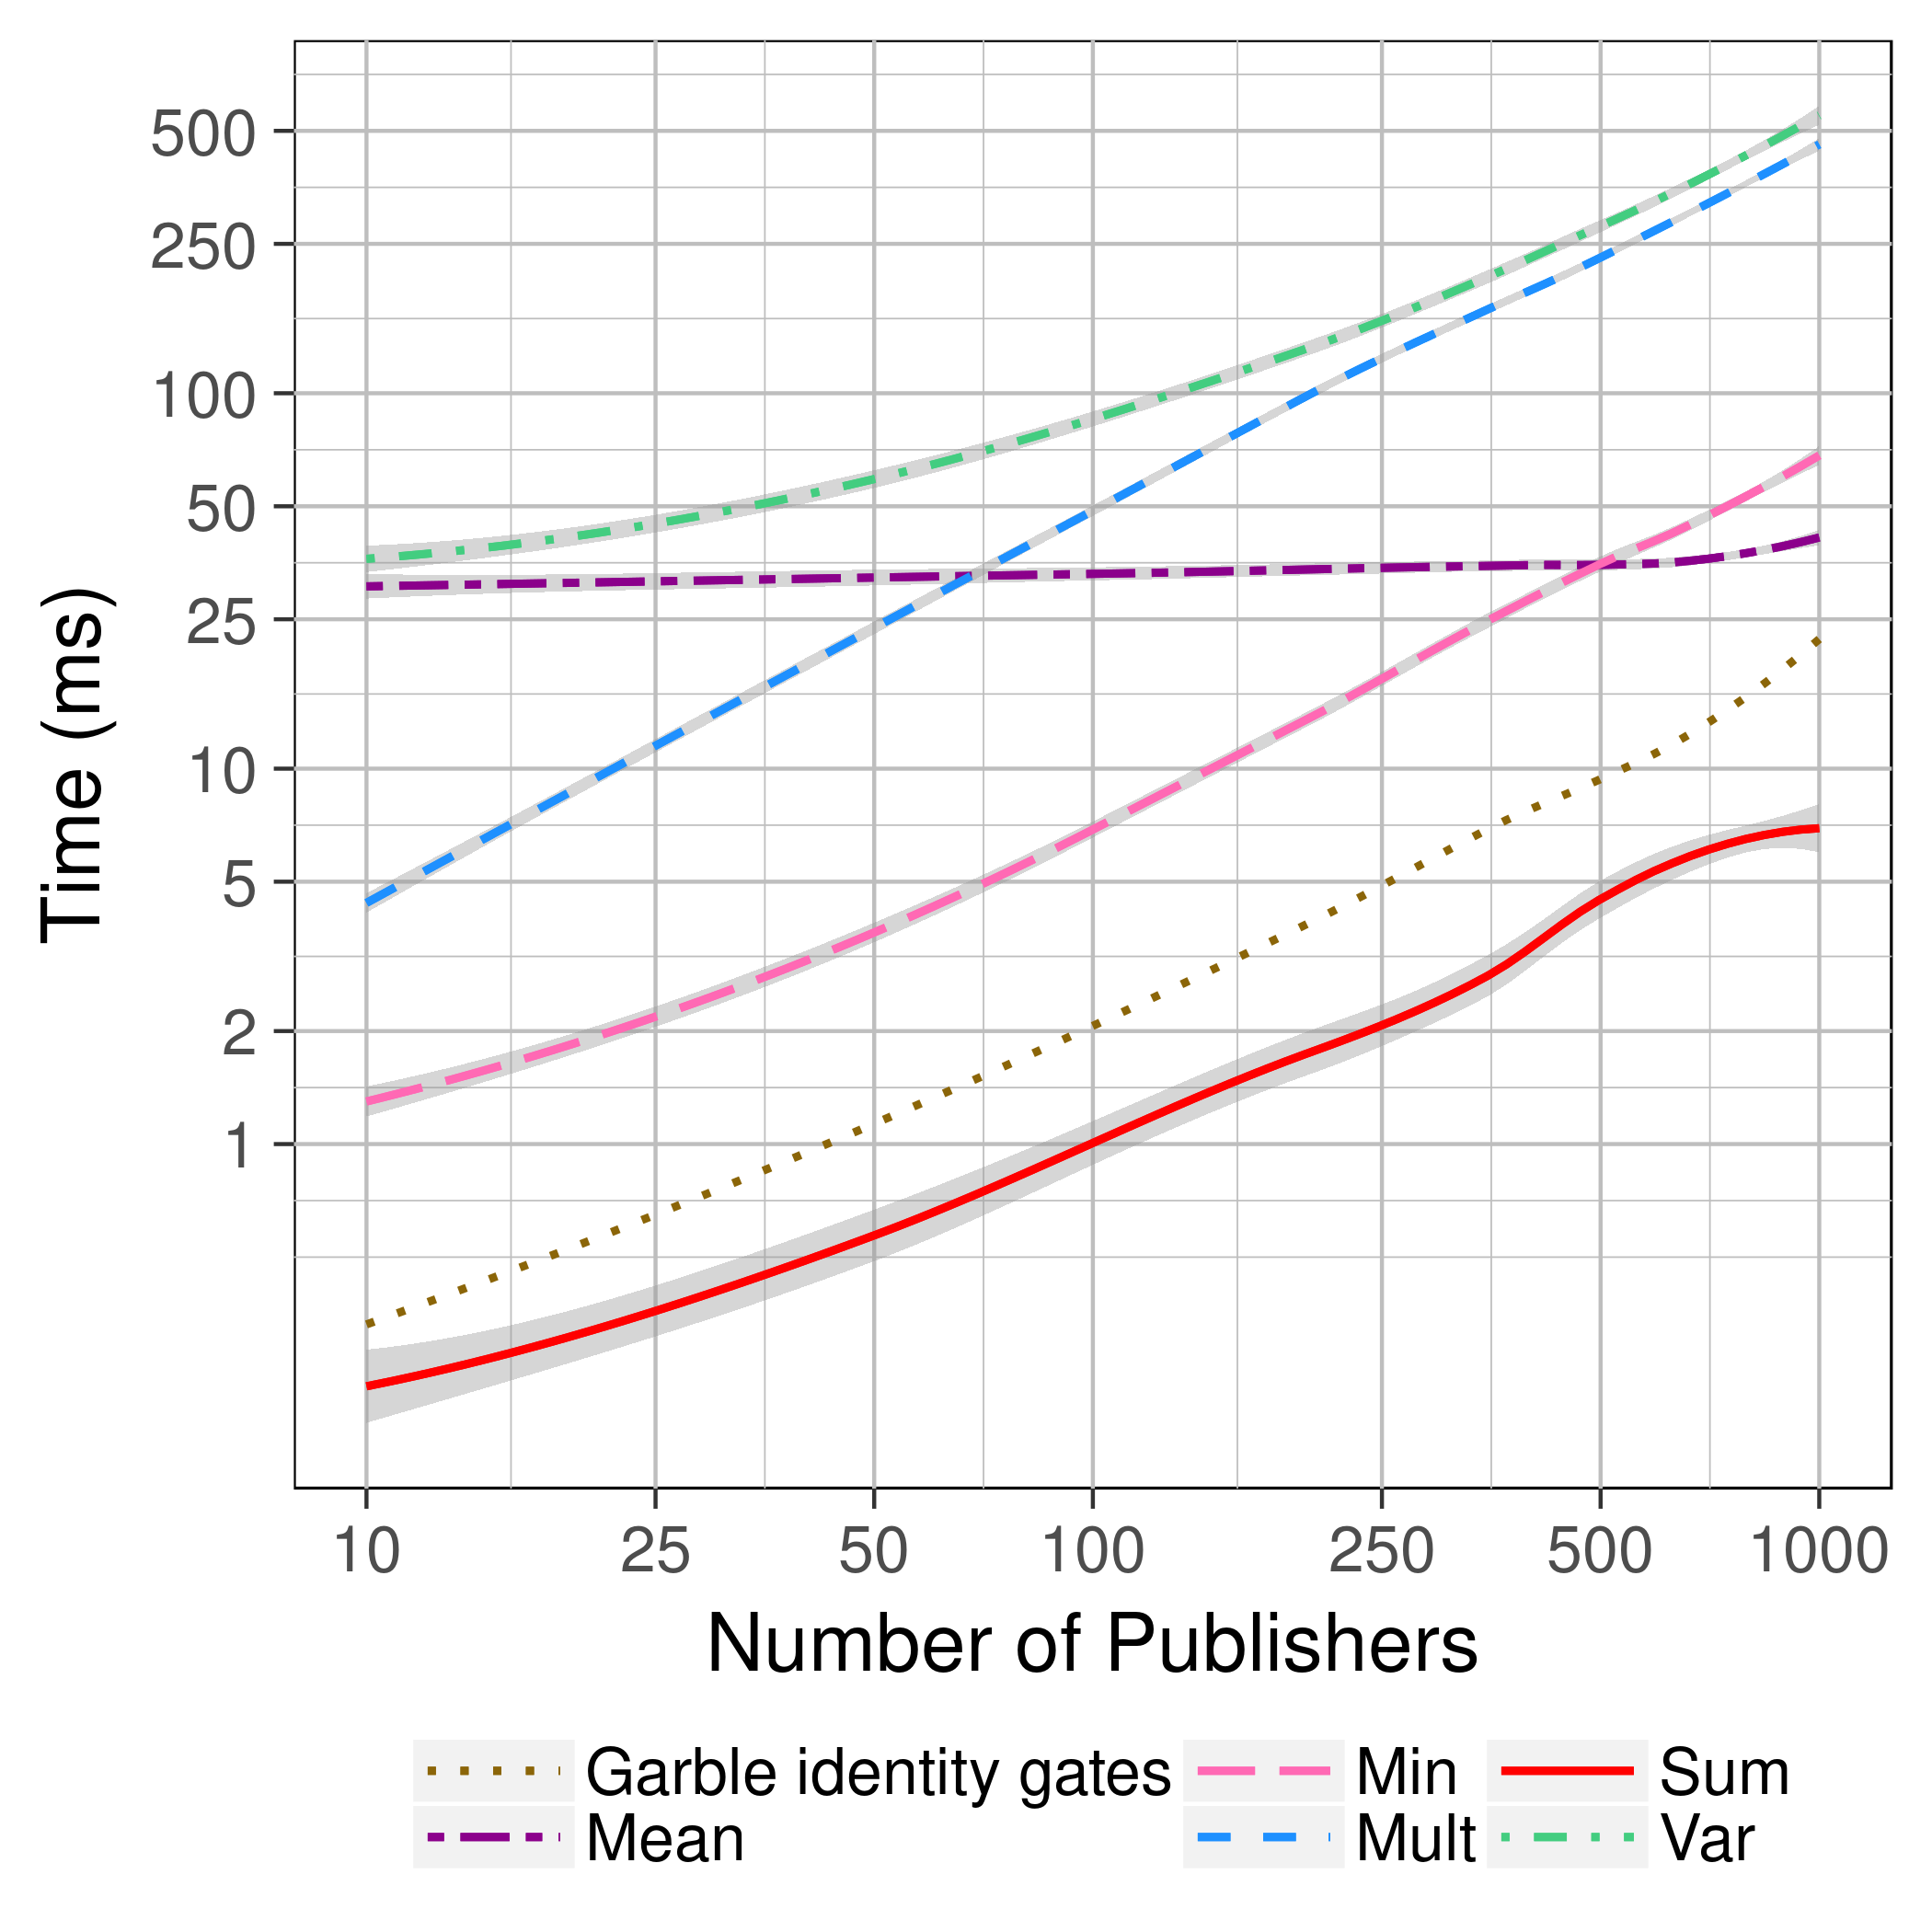
\includegraphics[width=\textwidth]{plots/eval_loglog.png}
        \caption{Evaluate}
        \label{fig:micro-eval-time}
    \end{subfigure}
    ~ %add desired spacing between images, e. g. ~, \quad, \qquad, \hfill etc.
    \begin{subfigure}[b]{0.32\textwidth}
        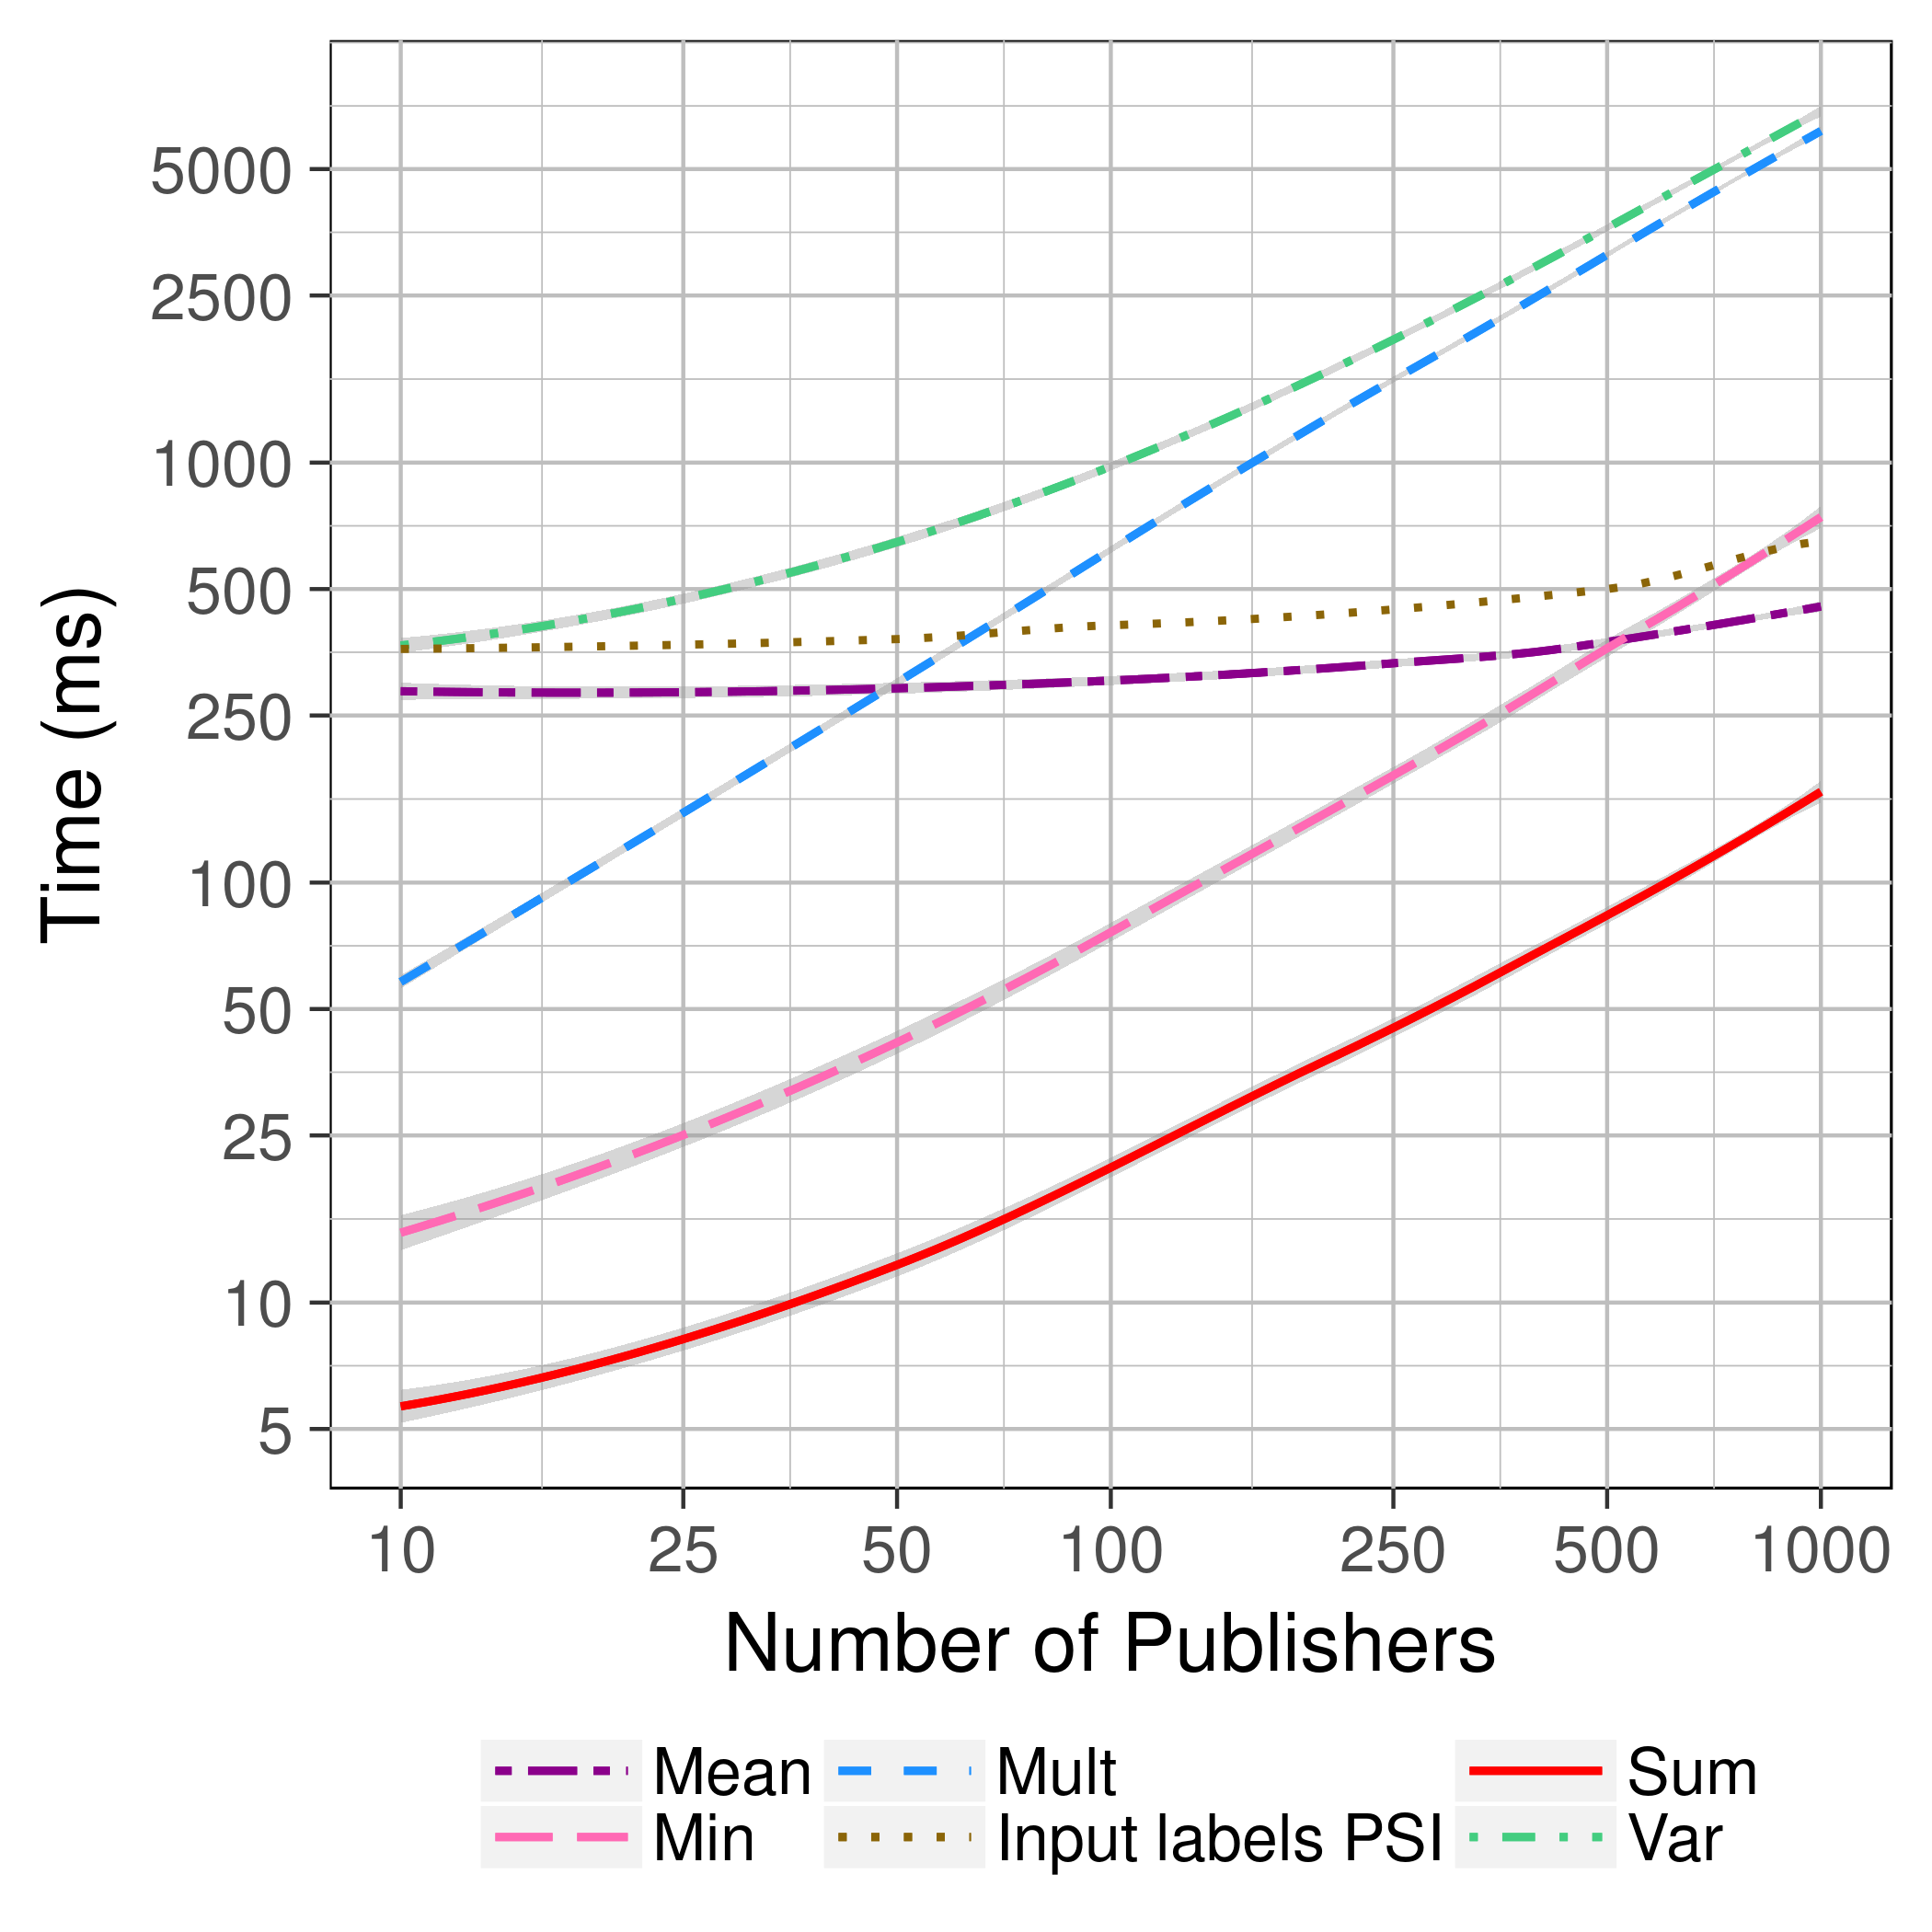
\includegraphics[width=\textwidth]{plots/send_loglog.png}
        \caption{Send}
        \label{fig:micro-send-time}
    \end{subfigure}
    \caption{Mean time required for garbling, evaluating and sending the
      garbled circuit to the \broker for each function in the microbenchmark.
      Results obtained from the mean of 5 repetitions for each configuration,
      with the confidence interval of 95\% shown in gray.}
    \label{fig:micro-times}
\end{figure*}

We have selected 5 numerical operations of varying complexity (\emph{summation,
multiplication, mean, variance, minimum/maximum}) to evaluate the cost of the
different parts of our implementation.  We securely evaluate these functions
over the values (encoded as 32 bit fixed point numbers) received from a
variable number of Publishers.

In figure~\ref{fig:micro-times} we show the timing results for the most
relevant steps of the secure computation happening between the \broker and the
\garbler of the 5 numerical operations for varying number of Publishers from 10
to 1000.  In particular, since we are encoding the Publishers values with 32
bits, the number of input wires will be the number of Publishers times 32.  We
would expect the evaluated functions to scale linearly in the three analyzed
steps of the protocol.  Whereas the \emph{multiplication} shows the more clear
linear scaling, other operations show a transitive state tending to linear,
with the most extreme case happening on the \emph{mean}.  We attribute this
later result to the fixed cost of the final division in the mean, which becomes
the dominant overhead of the circuit until the number of Pulbishers start
reaching the 1000.  On the other hand, the \emph{summation} is the most
lightweight function, and doesn't show yet a stabilizing linear trend for the
number of Publishers used in the experiment.  Accompanying the garble
(figure~\ref{fig:micro-garble-time}) and the evaluate
(figure~\ref{fig:micro-eval-time}) we show the time it took to garble and
evaluate the input identity gates.  We have also decoupled the time spent
following the Private Set Intersection between the \broker and \garbler from
the sending time, and we show it in figure~\ref{fig:micro-send-time}.

We can see that the time spent dealing with the identity gates (encrypting and
decrypting the inputs) makes a significant influence in the faster functions,
being comparable in magnitude to the evaluation and garbling time of the
\emph{summation} (the input decryption time is even higher than the garbled
circuit evaluation time for \emph{summation}).  We attribute this behavior to
the fact that this part of the protocol is implemented in Go instead of C like
the garbling and evaluation.

We can also see how the time spent on the Private Set Intersection protocol is
higher than the time required for sending in the case of the \emph{Mean},
\emph{Min} and \emph{summation}, although it seems that it will scale better
than the later two functions when the number of Publishers well passes the
thousands.

\begin{figure}
  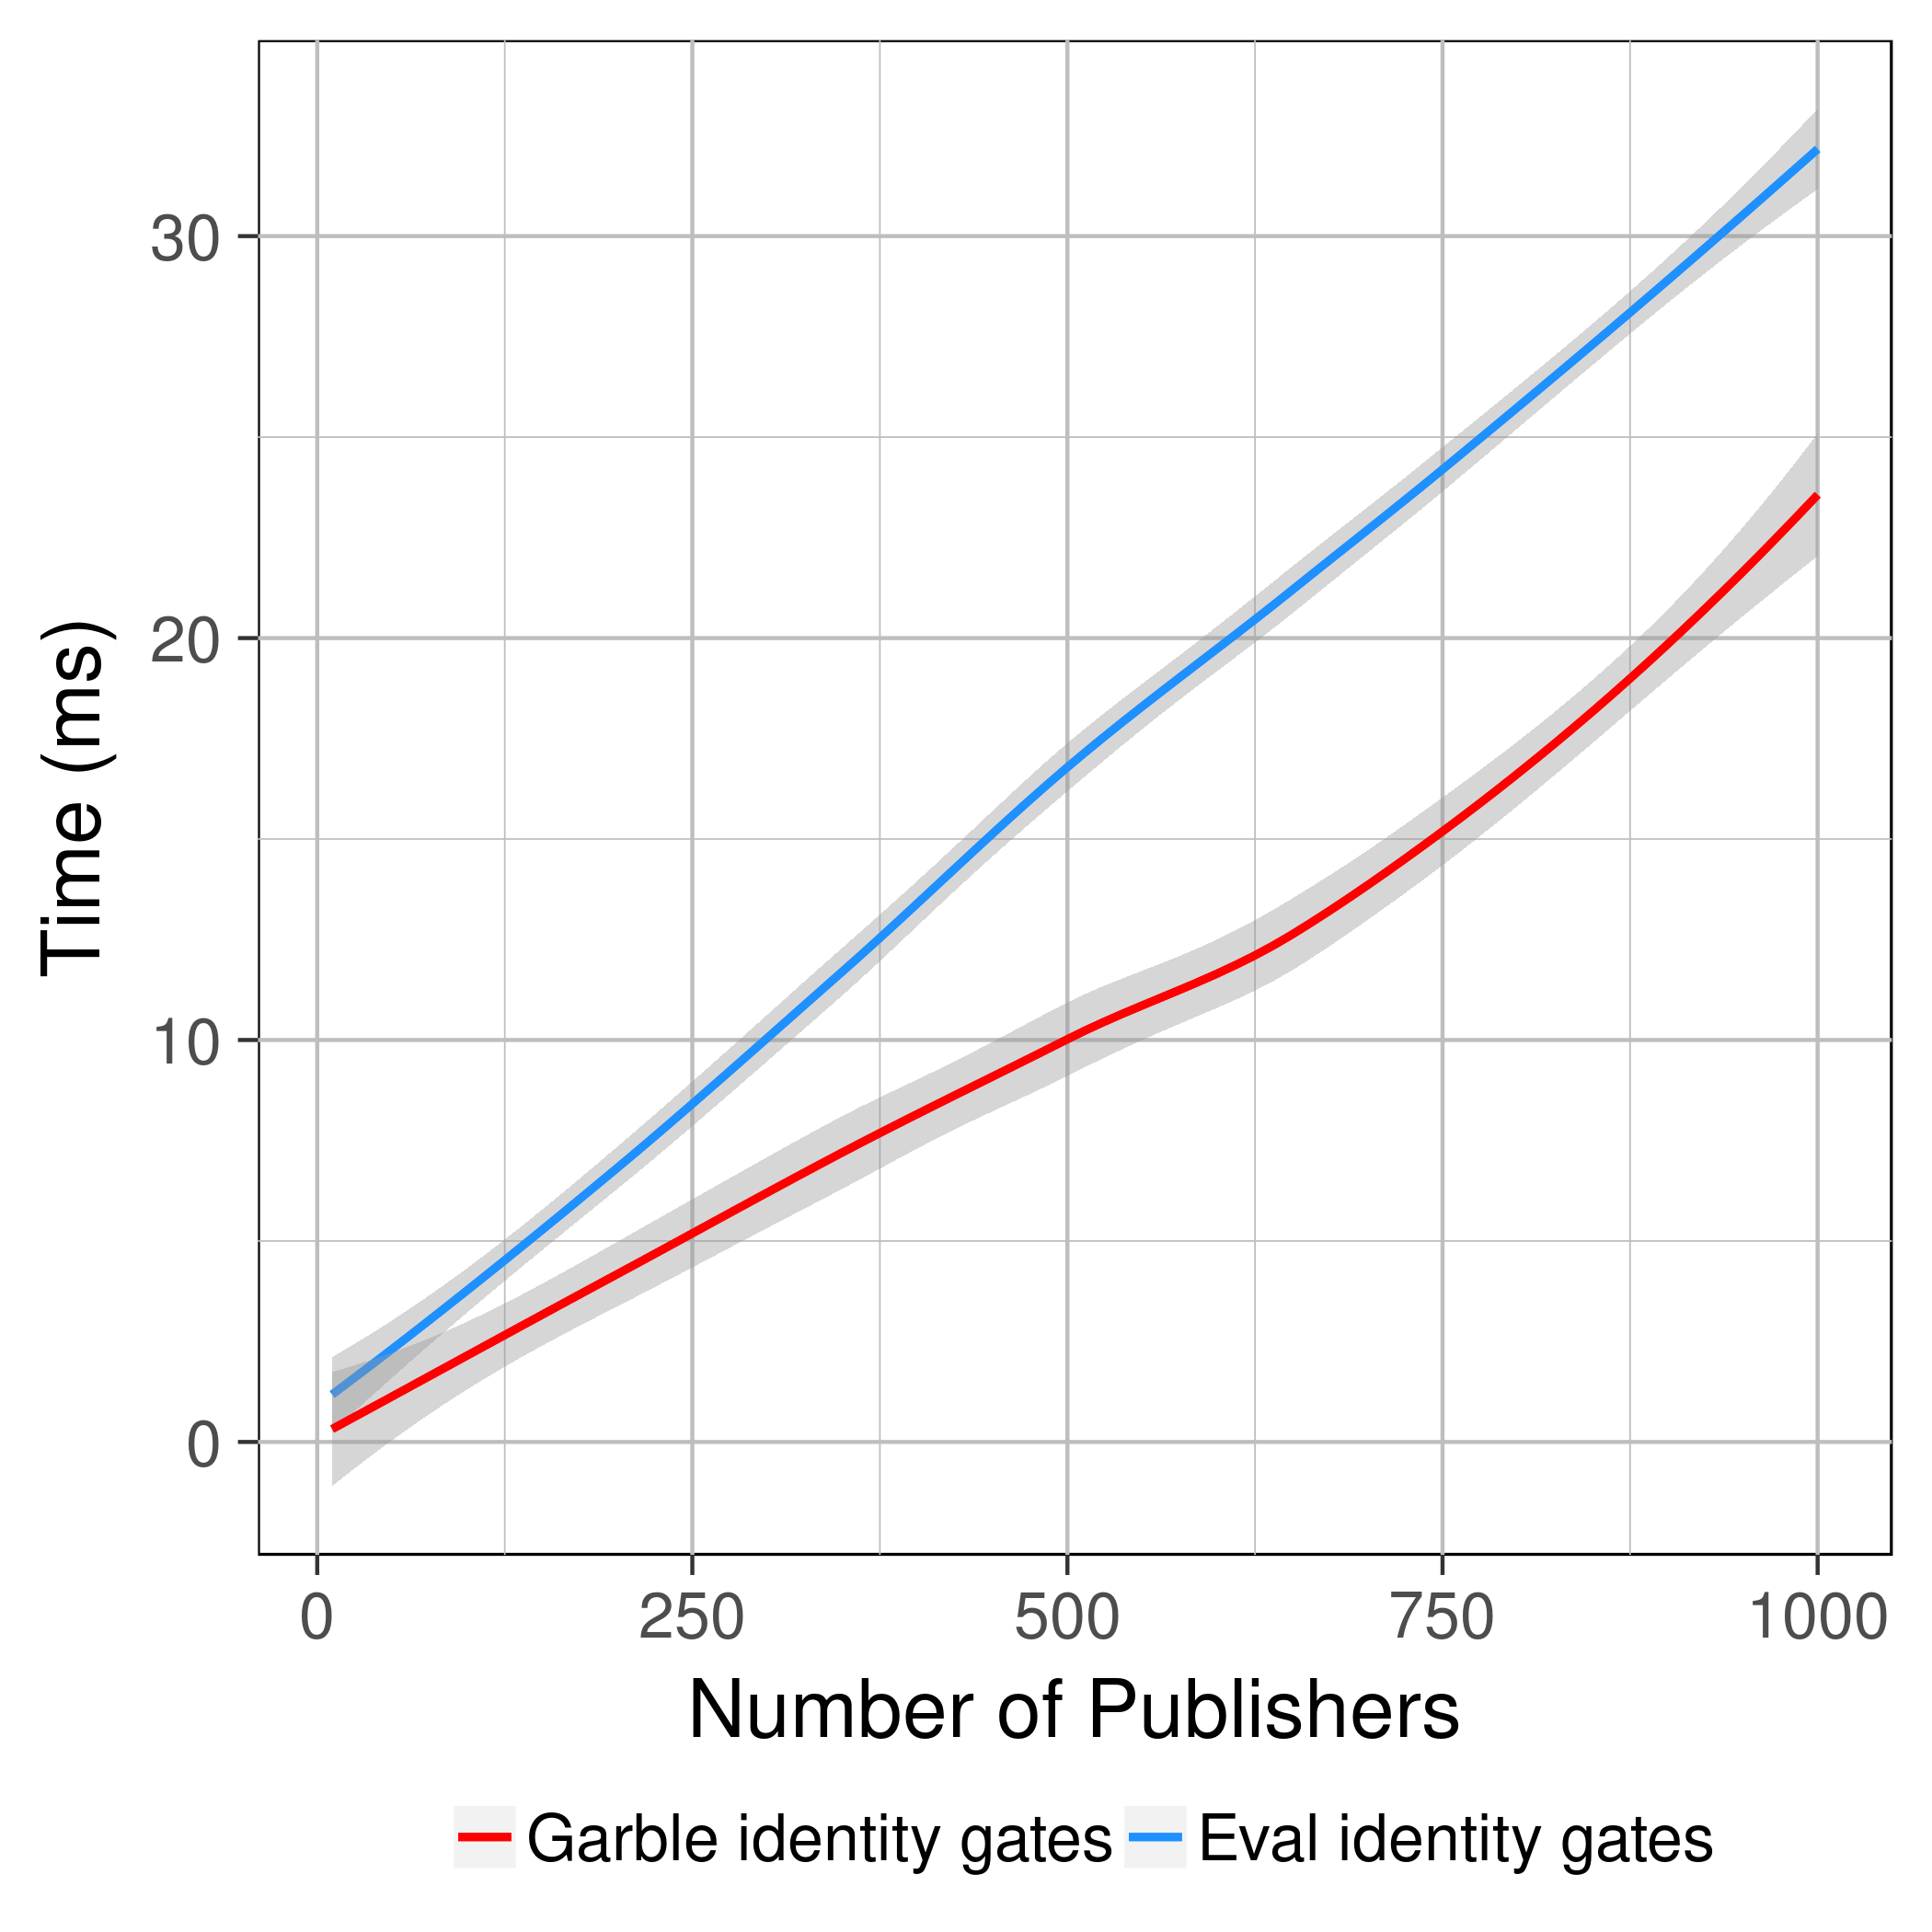
\includegraphics[width=0.32\textwidth]{plots/enc_dec.png}
  \caption{Time spent garbling and evaluating the identity input gates.
    Results obtained from the mean of all microbenchmark functions with 5
    repetitions each, with the confidence interval of 95\% shown in gray.}
  \label{micro-inputs}
\end{figure}

We can see in more detail a comparison of the time spent on garbling and
evaluating the identity gates in figure~\ref{micro-inputs}.  We expected the
garbling to be roughly twice the times of evaluating (garbling involves
encrypting two labels whereas evaluating involves decrypting one)

\begin{figure}
  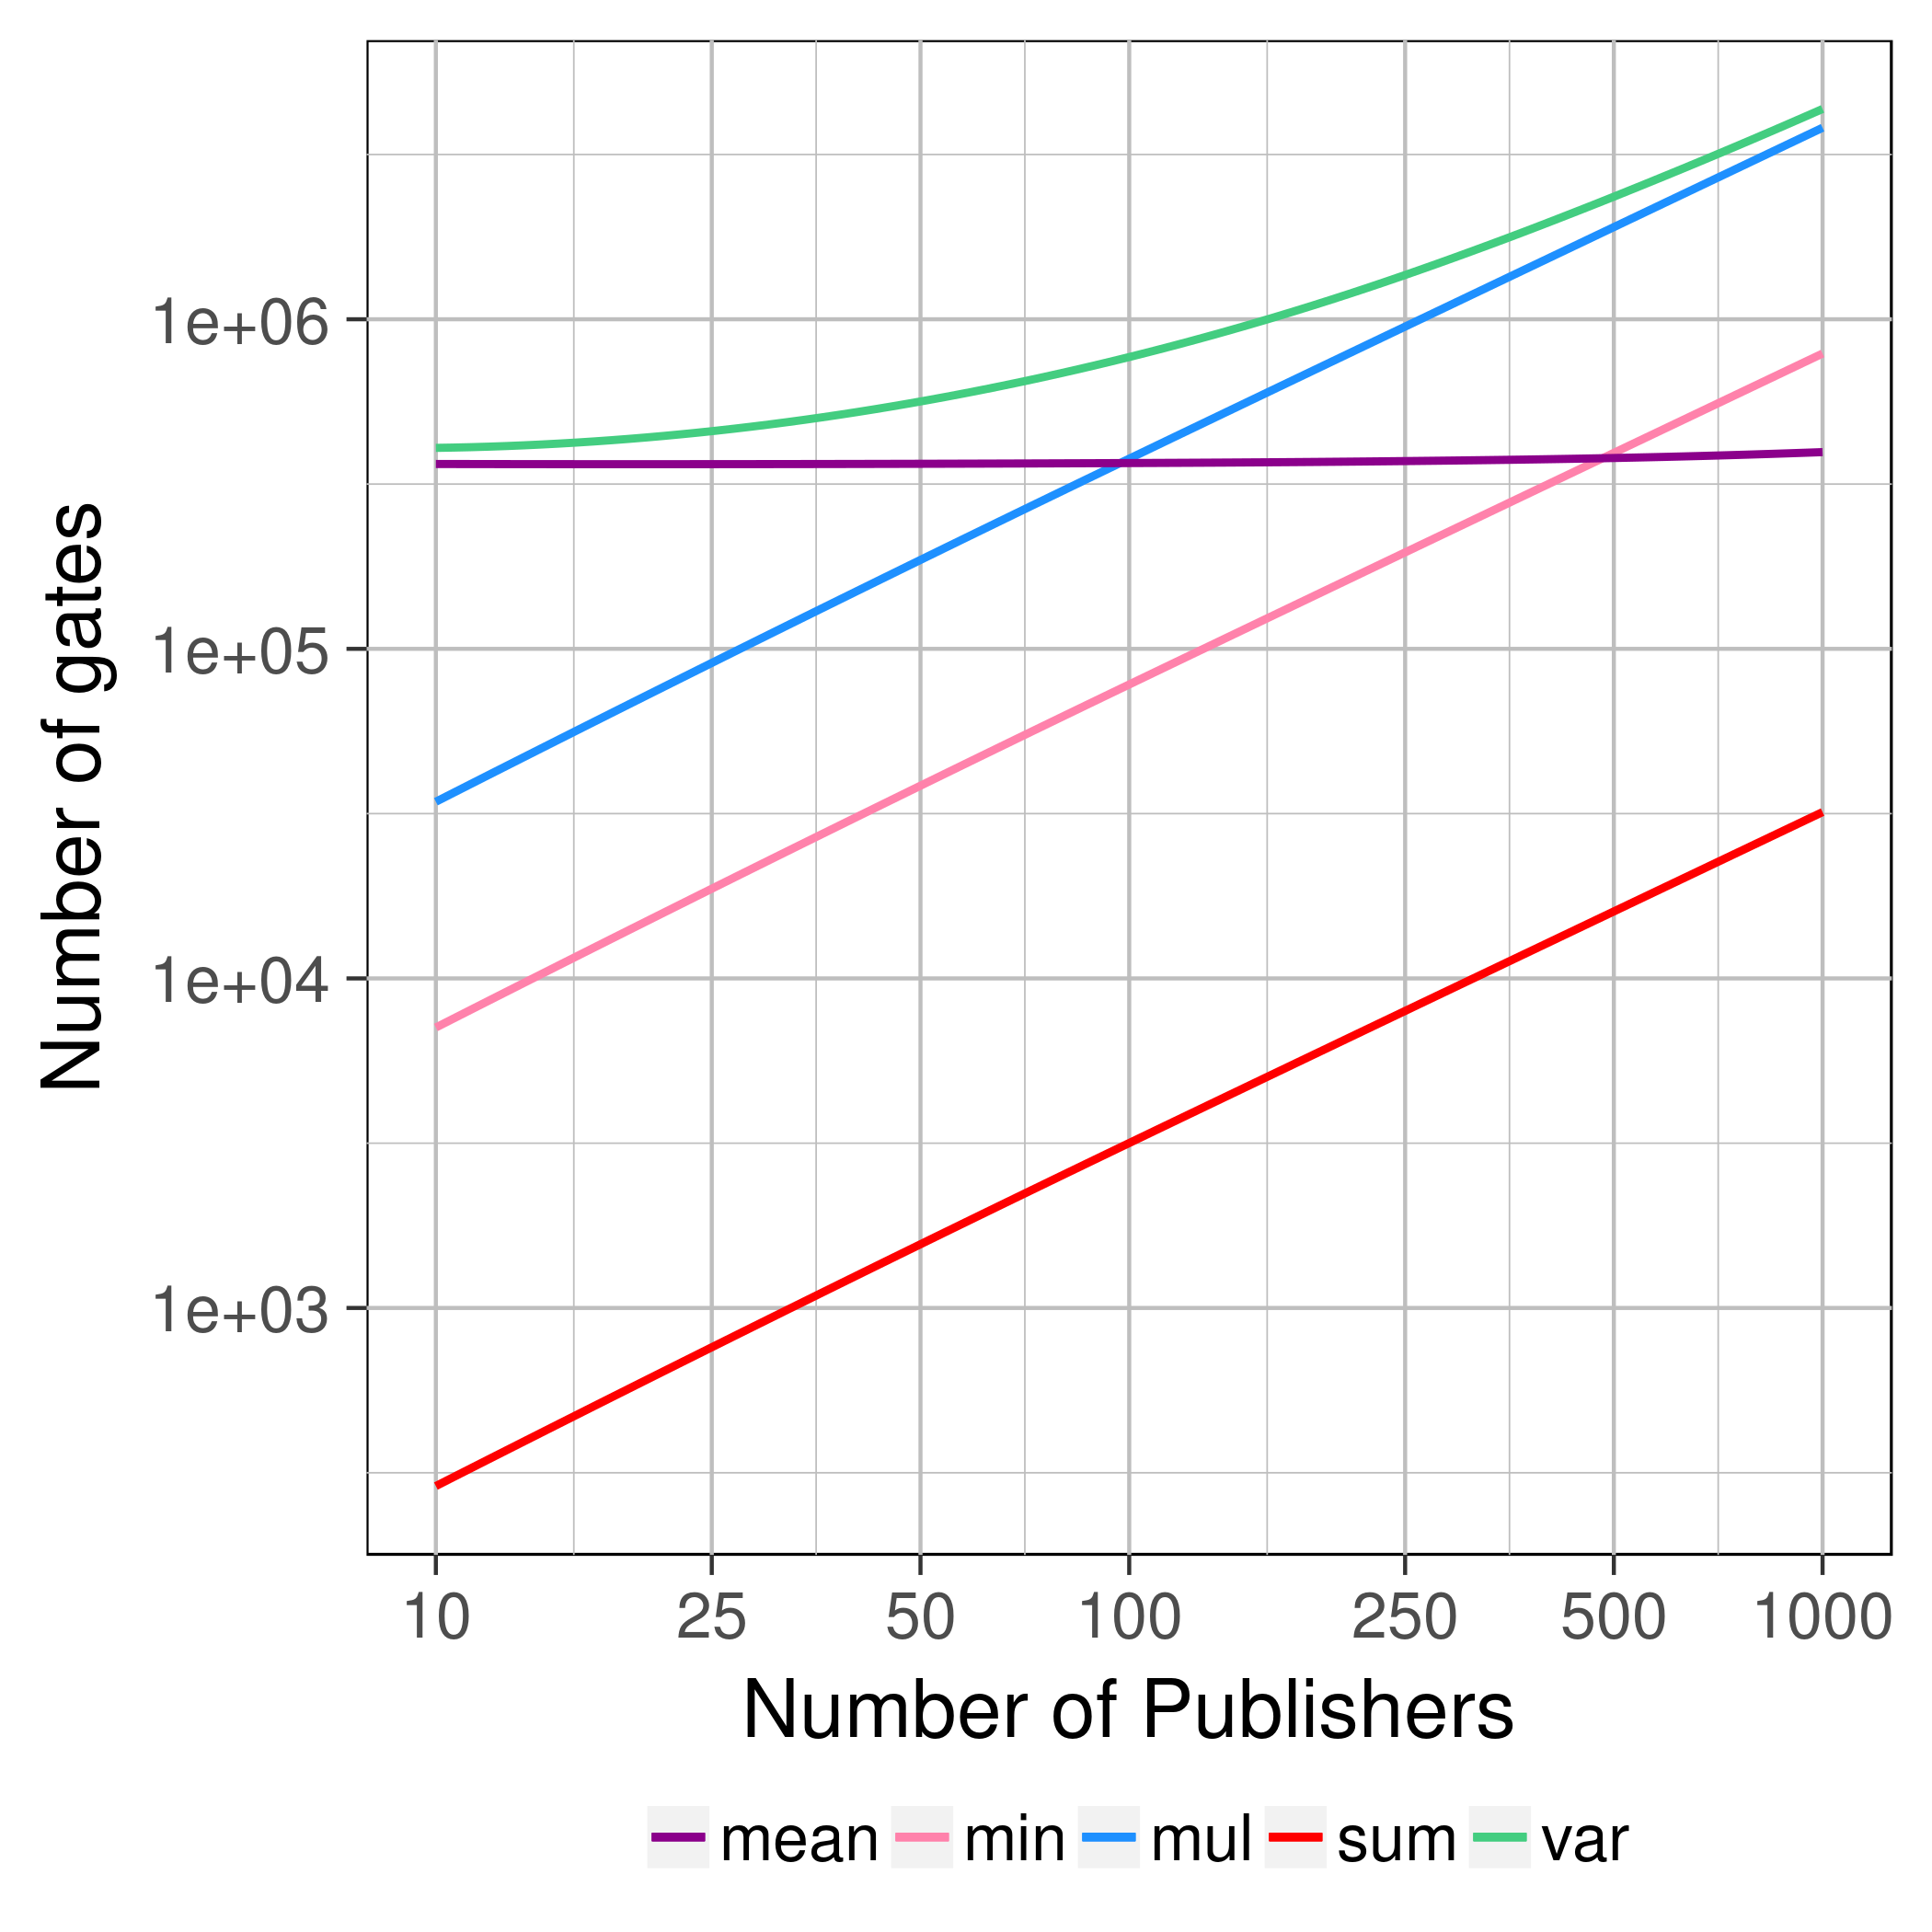
\includegraphics[width=0.32\textwidth]{plots/nonxor_gates_log.png}
  \caption{Non-XOR gates count per function used in the microbenchmarks.}
  \label{micro-nonxor}
\end{figure}

In figure~\ref{micro-nonxor} we show the number of non-XOR gates (that is, the
gates that incur a garbling and evaluating and that increase the size of the
garbled circuit) for every function.  We can clearly see the relation between
the number of the non-XOR gates and the cost of computing every function by
comparing shape of the plot with timing results shown in
figure~\ref{fig:micro-times}.

\begin{figure}
  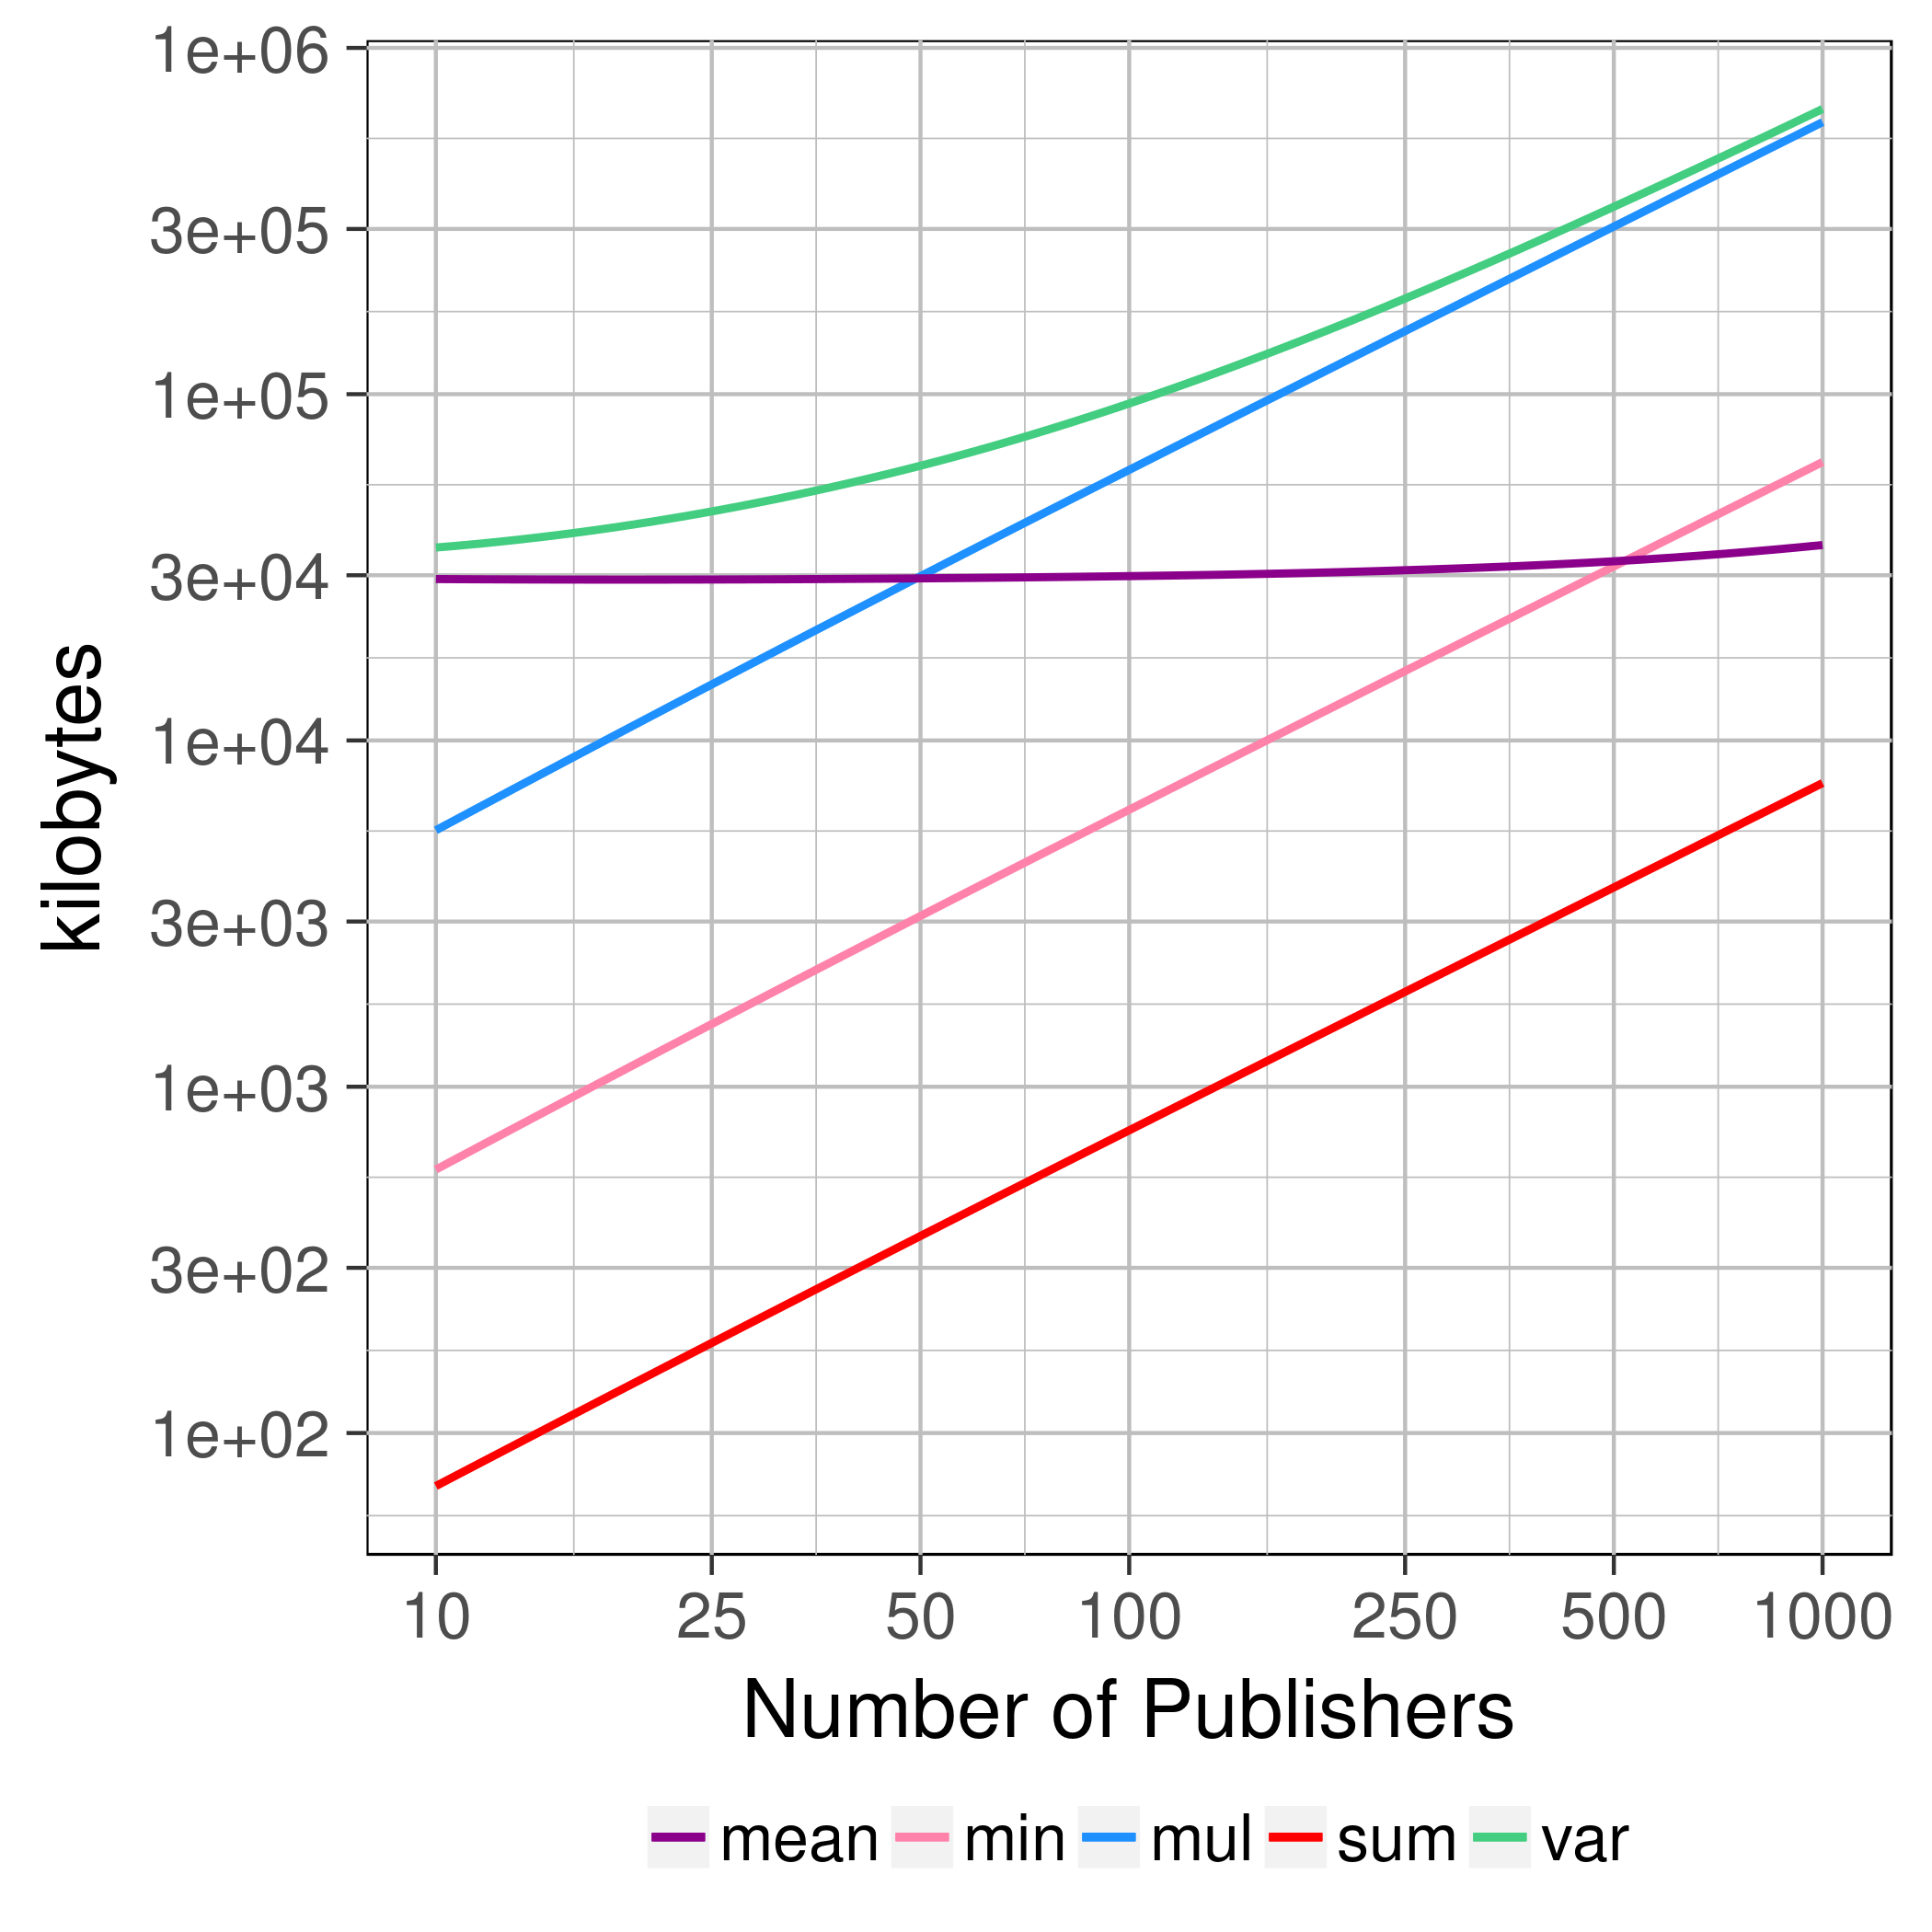
\includegraphics[width=0.32\textwidth]{plots/size_log.png}
  \caption{Size of the garbled circuit and the associated date required by the
    \broker to evaluate it.}
  \label{micro-sizes}
\end{figure}

In figure~\ref{micro-sizes} we see the transfer size between the \broker and
the \garbler for every function (that is, the size of the garbled circuit and
the associated data structures like the masking round used).  As expected, the
shape is very similar to the number of non-XOR gates for function shown in
figure~\ref{micro-nonxor}.  In the figure we can observe where the bottleneck
of using garbled circuits come from: the need to transfer such amount of data
over the network.  This fact makes the choice of network bandwidth between the
\broker and the \garbler critical, leading to very different results in
performance (which is dominated by the sending time) depending on the choice.
This figure also helps us understand the limits of using garbled circuits: the
\emph{variance} and \emph{multiplication} garbled circuits for 1000 Publishers
sizes are close to 700 MiB; considering the linear scaling we can easily
predict the point where the garbled circuits would be too big to fit into the
computer memory.

\begin{table}
    \begin{tabular}{l|*{4}{c}c}
      & \textbf{Sum} & \textbf{Mult} & \textbf{Mean} & \textbf{Var} & \textbf{Min/Max} \\
    \hline
    \textbf{Reduction} & 06.63 \% & 09.76 \% & 06.87 \% & 09.68 \% & 14.47 \% \\
    \end{tabular}
    \caption{Number of gates reduction for each microbenchmark function we
      would obtain by using the half-gates optimization.}
    \label{micro-and}
\end{table}

Considering the fact that we are not using the half-gates size optimization in
our garbled circuits, we show in table~\ref{micro-and} the reduction we would
observe for the experiments with 1000 Publishers if we had used such
optimization (computed by counting the number of AND gates used in each
circuit).  We observe the biggest reduction in the \emph{Min/Max} functions,
leading us to conclude that implementing the half-gates optimization would be a
clear improvement overall by reducing the sending time of the garbled circuits.

\vspace{-4pt}
\subsection{Applications}

We have prepared 3 concrete applications based on real IoT datasets to show
possible real usages of the presented protocol.

% Turonet, wireless propagation constant, linear regression
\smallskip
\noindent\textbf{Wireless propagation constant}

\noindent In this application we take the real time data provided by a testbed of IoT
nodes deployed in our university forming a mesh network.

The mesh network is formed by a fixed number of nodes deployed in different
static locations in the same building that connect to each other via wireless.
Every node tries to connect to the others unless they are too far, giving us an
upper bound of $n \cdot (n-1)$ connections where $n$ is the number of nodes.
Each node periodically publishes the received signal strength ($RSS$) in dBm of
the nodes it is connected to; and this measure can fluctuate over time due to
fading.

We are interested in estimating the wireless propagation constant ($\eta$) in
the medium while preserving the privacy of the nodes (that is, their location,
the distance between nodes and their reported signal strength measures).
The value of $\eta$ can be useful in characterizing the radio propagation
environment and performance of the network and it can be derived from the
following formula: \mbox{$RSS = -10 \cdot \eta \cdot log_{10}(distance) - C$}.
We will estimate $\eta$ by finding a linear model for the $RSS$-distances pairs
obtained from the nodes.

% This was my original interpretation.  Since we already have the experiments,
% let's move this to the Environmental Berkeley indoor sensing data, but leave
% the formula description and linear regression explanation here.
In particular, we perform a linear regression so that we can model the $RSS$ as
a linear combination of a logarithmic function of the distance.  To estimate
the parameters of the one dimensional linear model ($y = ax + b$) we use the
ordinary least squares technique, which gives us the following closed-form
formula:

\[
\begin{pmatrix} b \\ c \end{pmatrix} =
\left( \displaystyle\sum_{i=1}^n \begin{pmatrix} 1 \\ x_i \end{pmatrix}
  \begin{pmatrix} 1 & x_i\end{pmatrix}\right)^{-1}
\left( \displaystyle\sum_{i=1}^n y_i \begin{pmatrix} 1 \\ x_i \end{pmatrix}\right)
\]

Evaluating the formula requires an inversion of a $2 x 2$ matrix, which we perform
by following the analytic solution.

For the evaluation of this application we construct a virtual scenario which
simulates the IoT nodes by running one Publisher per node in a separate
computer.  The Publishers will publish the $log_{10}$ of the distances to their
peers as an initial step, allowing the \broker to store these values for some
time avoiding the constant retransmission of these constants.  After this, the
Publishers will be sending values at the same rate of the nodes in order to
obtain the same performance results we would get by using live data from the
actual testbed.  Following our protocol, we will be estimating the wireless
propagation constant periodically, using the values received form the
Publishers.  We will vary the number of Publishers to analyze how this
application scales (notice that the number of inputs for the linear regression
formula grows quadratically when the number of nodes increases linearly)

\begin{figure}
  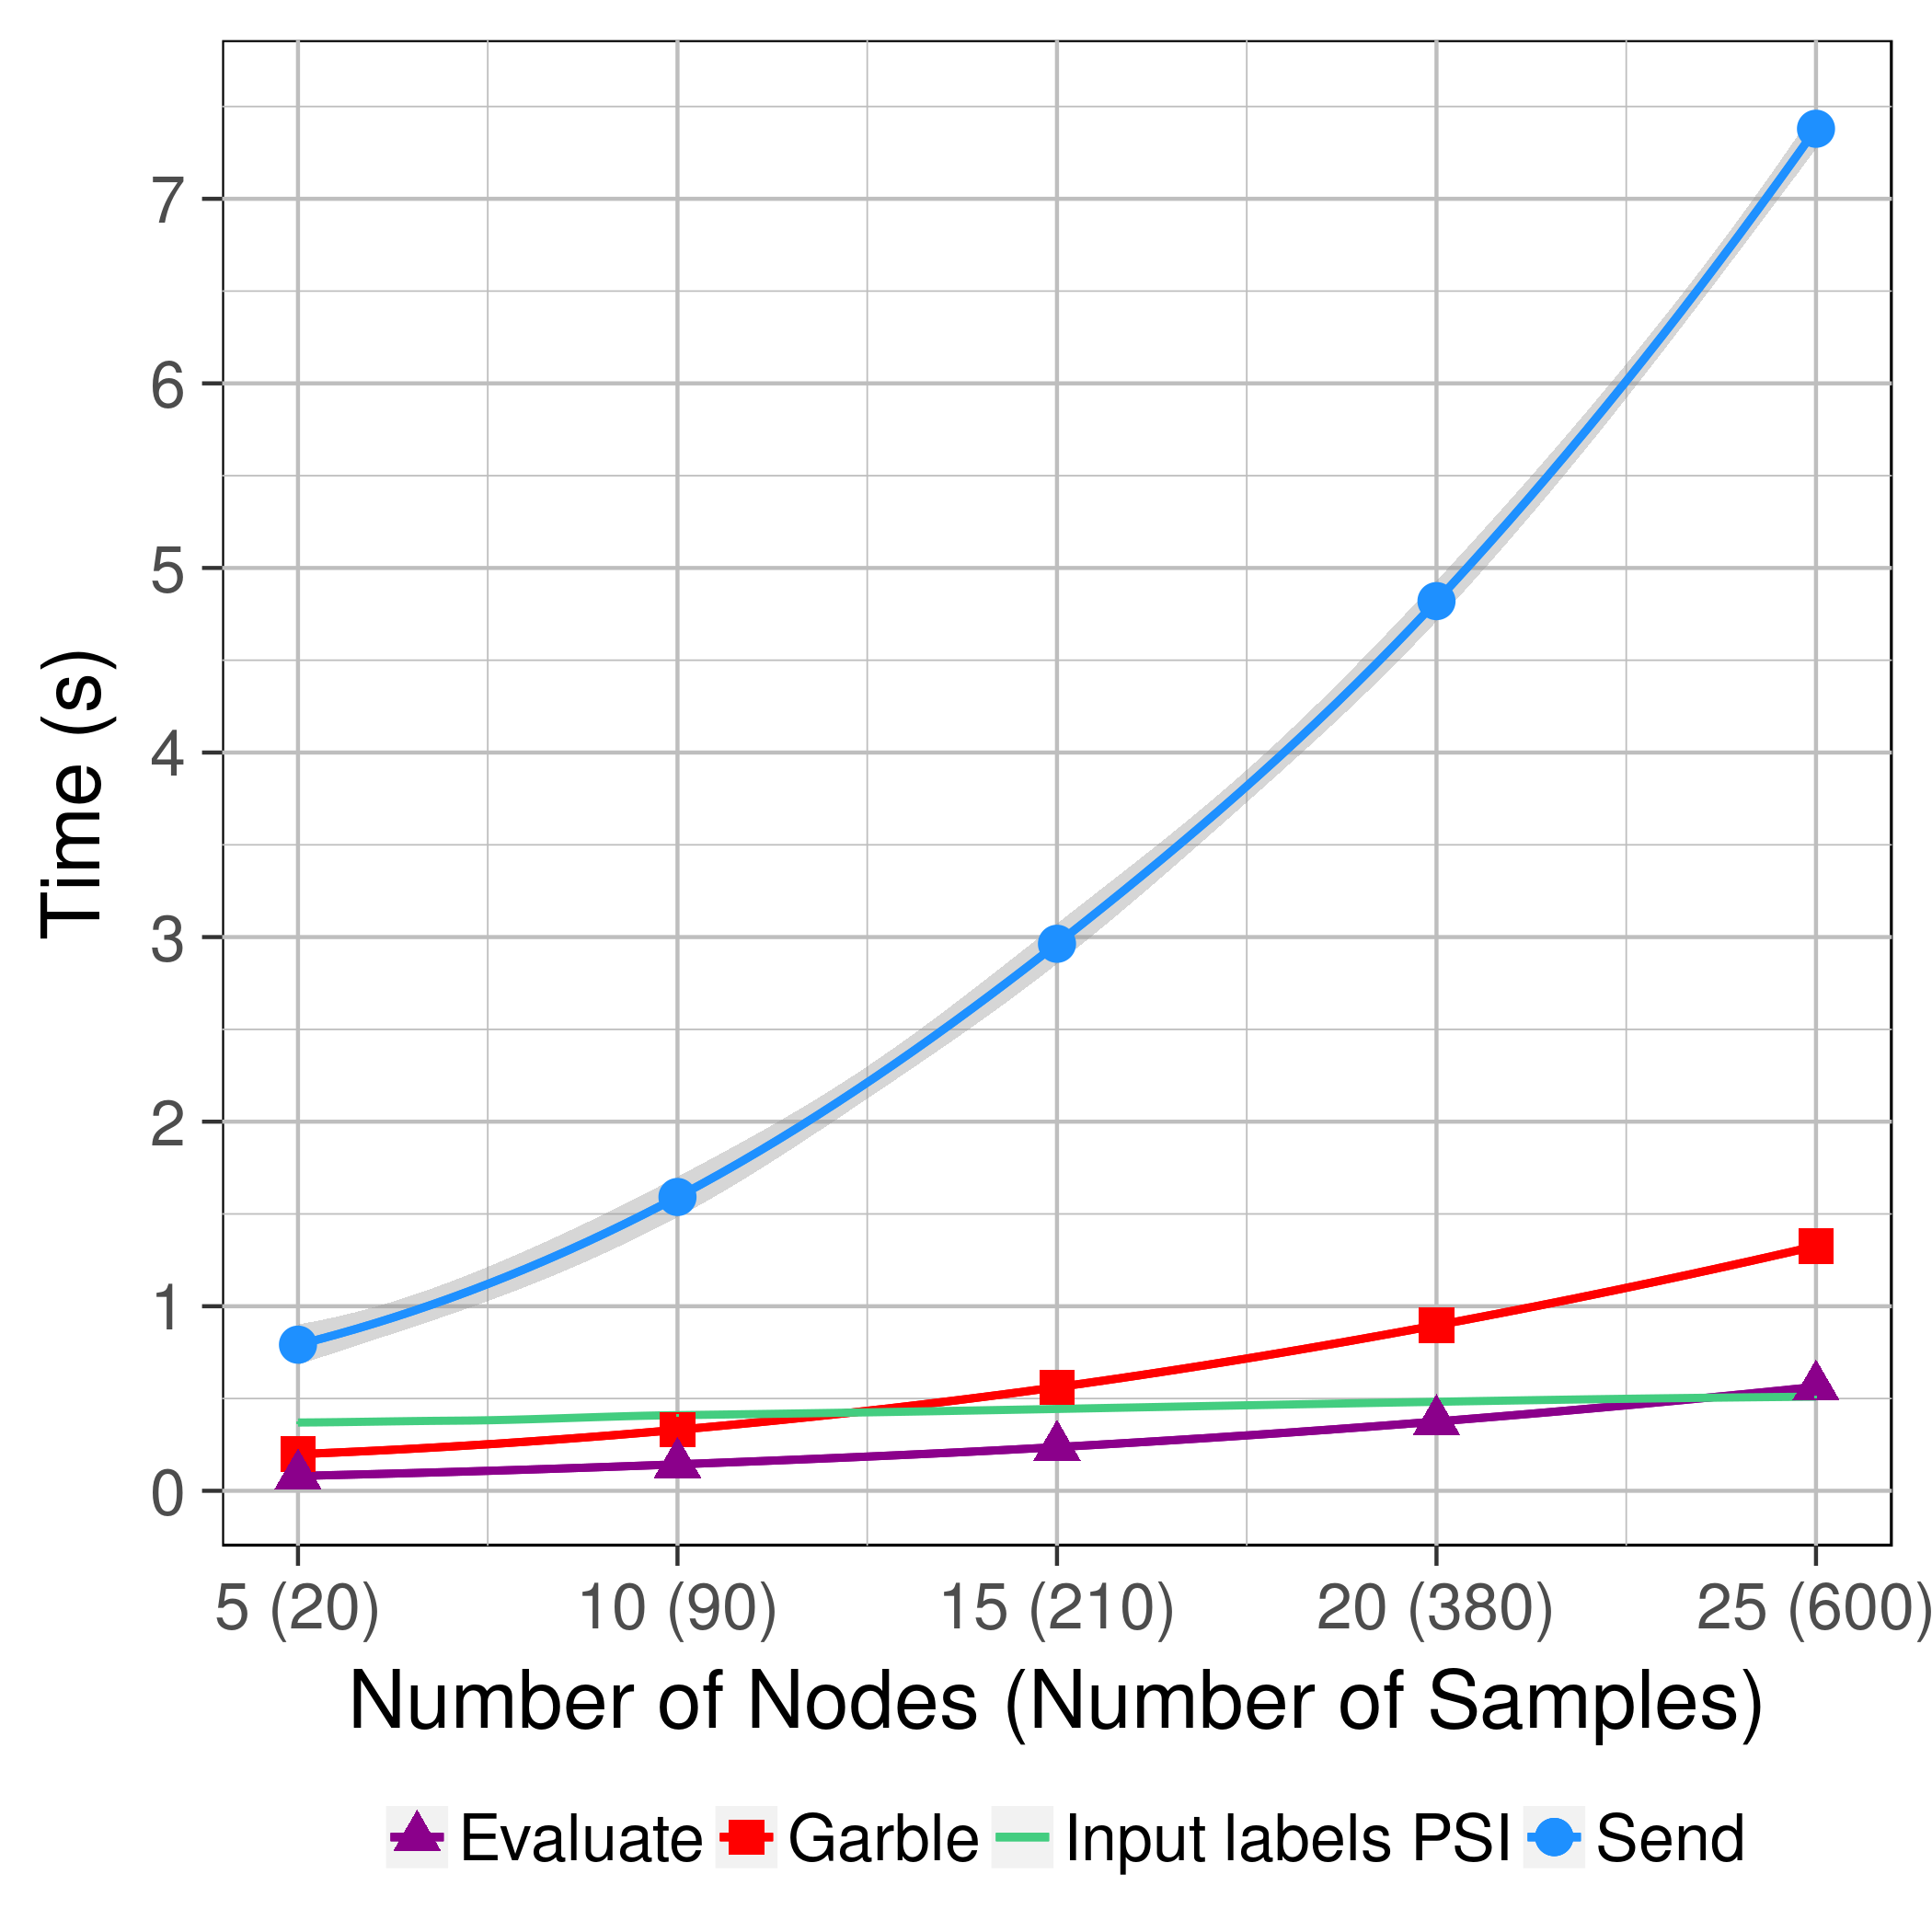
\includegraphics[width=0.32\textwidth]{plots/turonet.png}
  \caption{Mean time required for garbling, evaluating and sending the garbled
    circuit to the \broker for a varying number of nodes in the \emph{wireless
    propagation constant} application.  Results obtained from the mean of 5
    repetitions for each configuration, with the confidence interval of 95\% shown
    in gray.}
  \label{turonet-times}
\end{figure}

We show the results of the evaluation in figure~\ref{turonet-times}, where we
can clearly see that the cost for this application quickly grows with the
number of nodes.  Our experiments end at 25 nodes because at at 30 Nodes we
would be dealing with $30 \cdot 29 = 870$ samples to perform the correlation,
which corresponds to a garbled circuit of size bigger than 1 GiB.  At this
magnitude we hit a limit on the encoding used when marshaling the garbled
circuit in the Go RPC implementation, which doesn't support data structures
bigger than 1 GiB.  Notice however that we are using all the samples to
calculate the linear regression even though a random sample of a smaller size
would suffice; and that our scenario considers that all nodes are
interconnected, which will usually not be the case when the number of nodes
reaches a significant value.

% Environmental Berkeley indoor sensing data, correlation
\smallskip
\noindent\textbf{Correlation of environmental indoor sensing data}

\noindent For this application we will be using the environmental indoor sensing data
provided by the Intel Berkeley Research
lab\footnote{\url{http://db.csail.mit.edu/labdata/labdata.html} (accessed
2017-05-18)}.  This dataset provides 2.3 million readings collected
from sensors with the following values: temperature in degree Celcius, humidity
in percentage and light measured in Lux.

We are interested in finding relationships between pairs of data streams, each
coming from a different sensor, while maintaining the individual readings
private.

In this application's scenario, we assume that each sensor would be an
individual Publisher that sends readings periodically.  The \broker would
accumulates streams of published values from each sensor, and when requested,
the it would samples pairs of those streams at random over a specific period of
time to perform a correlation analysis between the two.  For our experiments we
vary the number of samples and simulate the application by supplying the \broker
with the given number of samples in a batch.

% Formula:
The correlation is a measure of statistical relationship among pairs of
variables in which higher value represents higher dependence.  Following the
Pearson's product-moment coefficient, we can measure the dependence between
samples of two variables (in our case, sensor readings) using the following
closed-form formula:

\vspace{-8pt}
\[
r_{xy} = \frac{\displaystyle\sum_{i=1}^n (x_i - \bar{x}) (y_i - \bar{y})}
{\sqrt{\displaystyle\sum_{i=1}^n (x_i - \bar{x})^2 (y_i - \bar{y})^2}}
\]

To improve efficiency, we evaluate the squared correlation ($r_{xy}^2$) to avoid
computing the square root in the function circuit, which would be an expensive
operation.

As a comparison, we will also evaluate the cost of computing the
one-dimensional linear regression over two streams of values with a varying
number of samples, which also gives us information about the relationship
between the two data streams.

\begin{figure}
  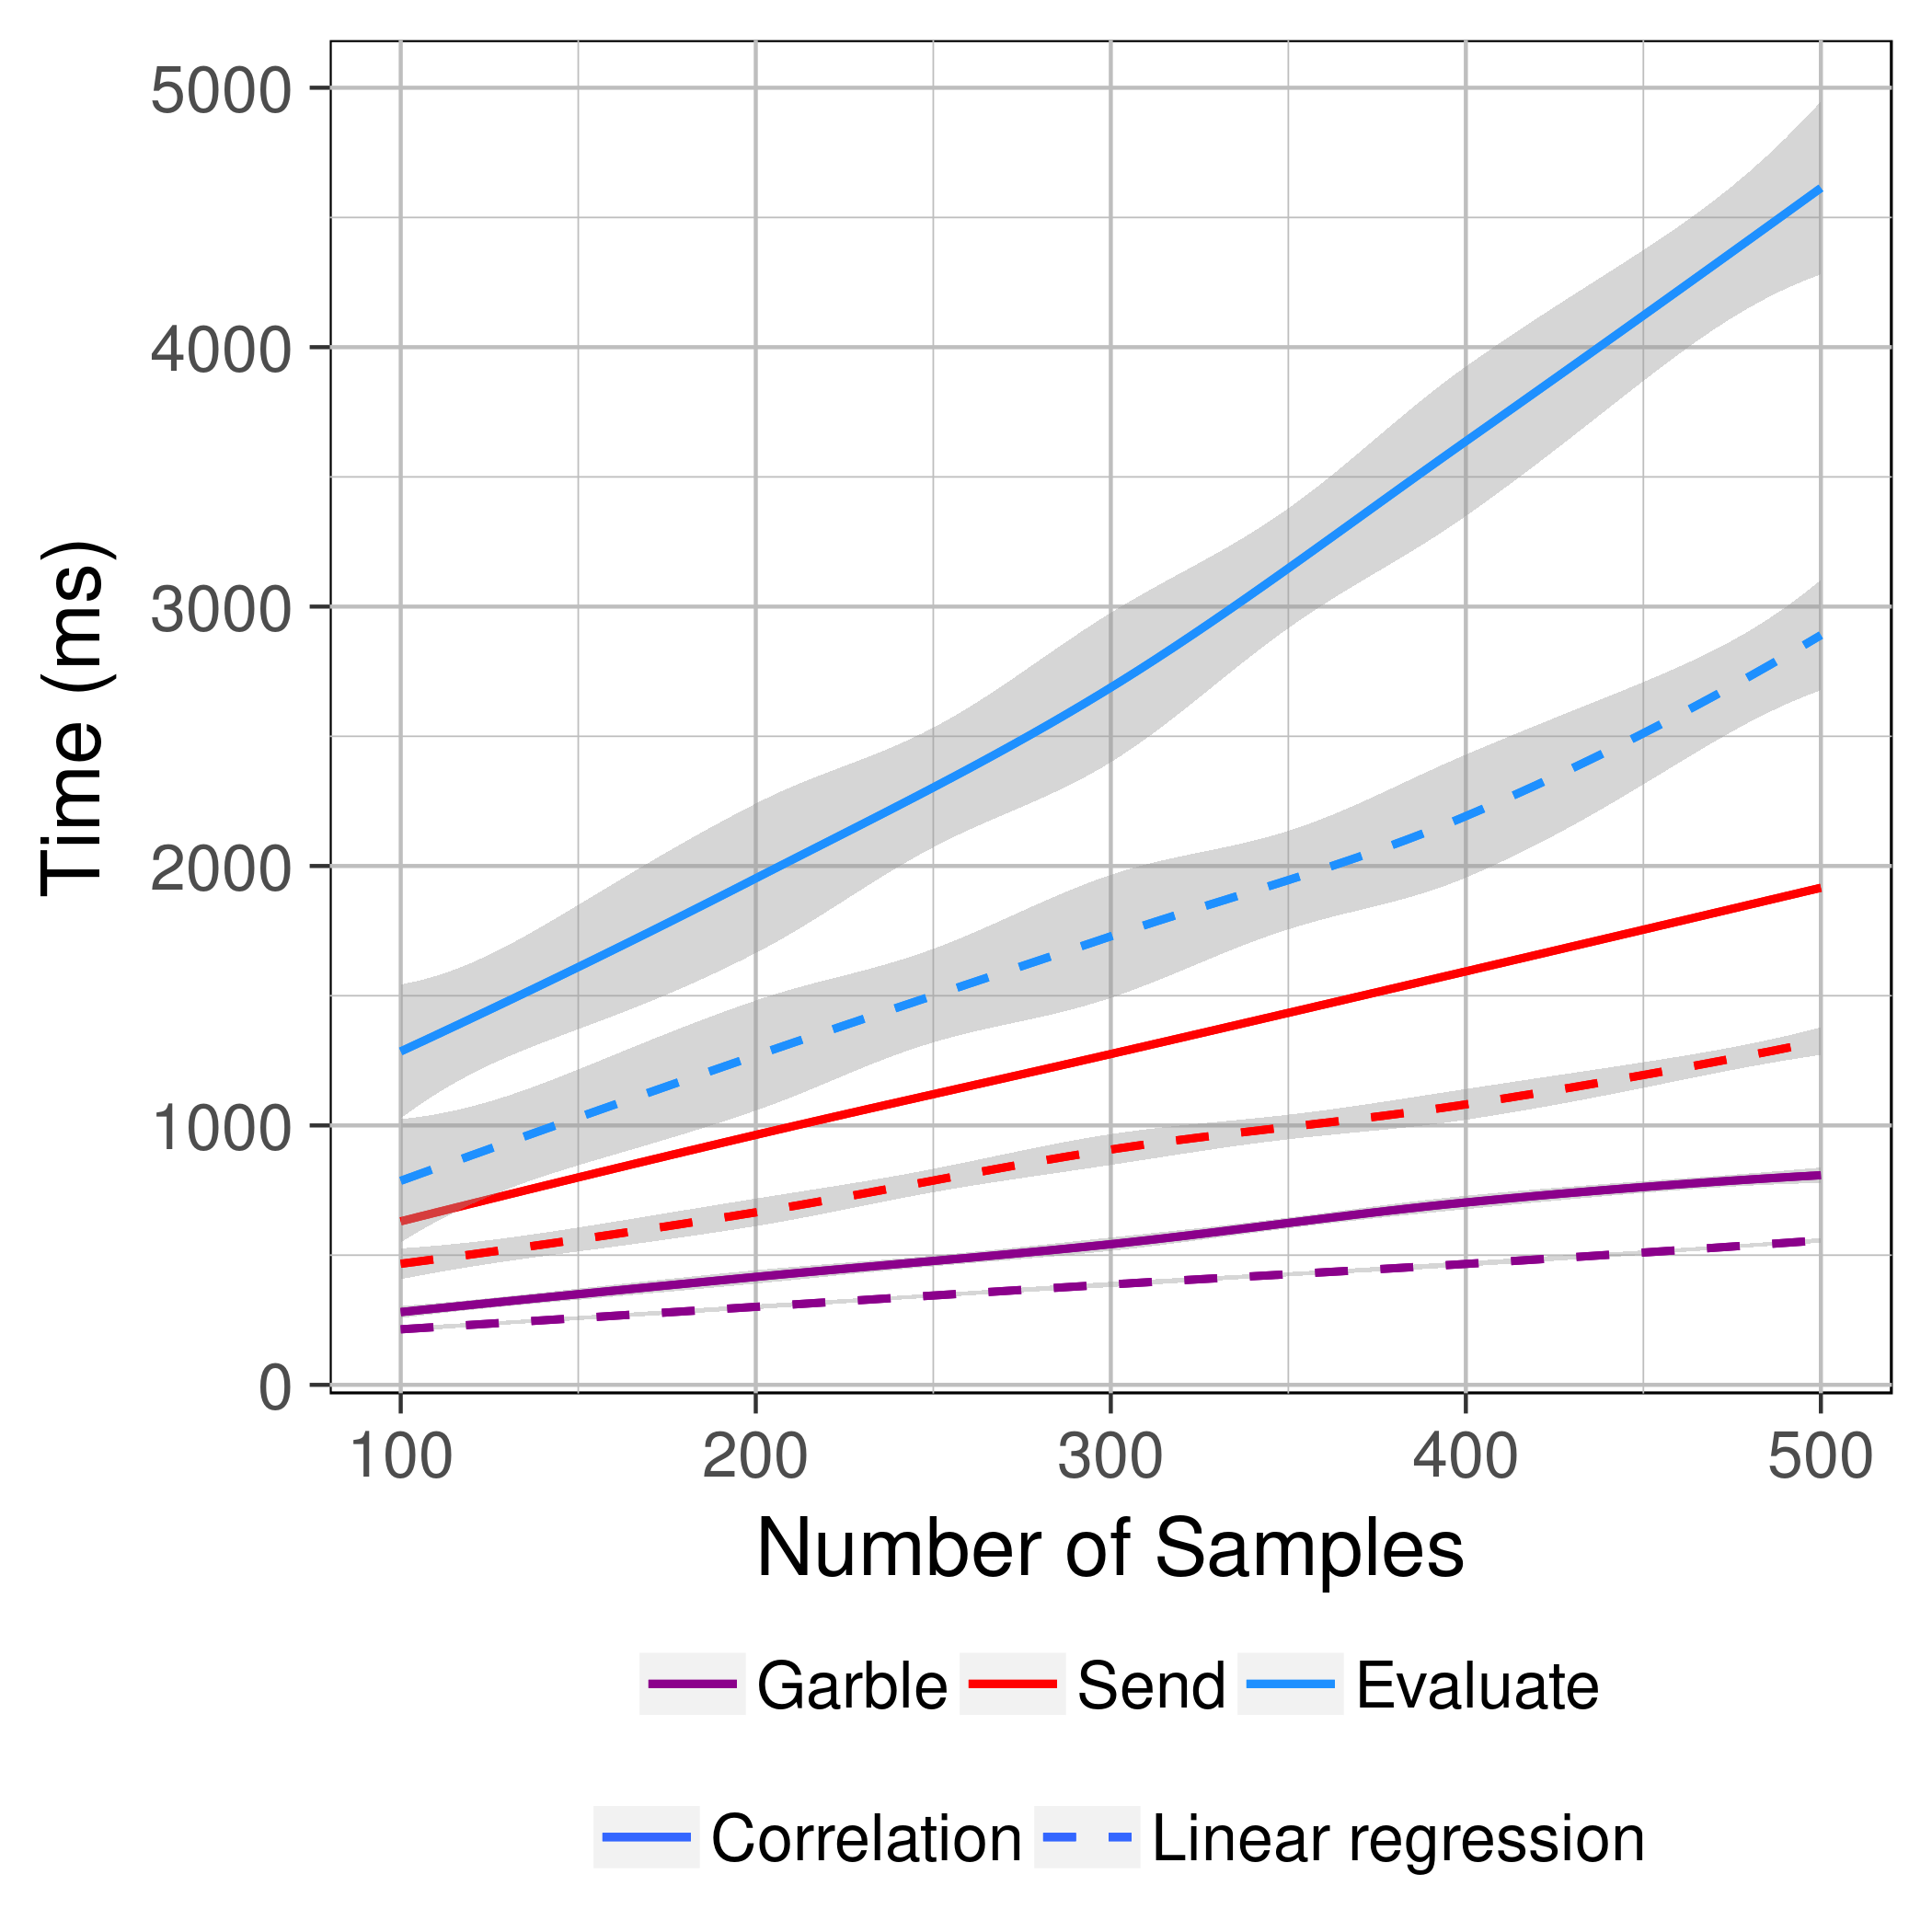
\includegraphics[width=0.32\textwidth]{plots/stream.png}
  \caption{Mean time required for garbling, evaluating and sending the garbled
    circuit to the \broker for computing the squared correlation and linear
    regression of data streams.  Garbling and evaluating includes the time to
    garble and evaluate the input identity.  Results obtained from the mean of
    5 repetitions for each configuration, with the confidence interval of 95\%
    shown in gray.}
  \label{stream-times}
\end{figure}

As we can see in figure~\ref{stream-times} the cost of computing the
correlation is roughly the double of the cost of computing the linear
regression.  Taking this result into consideration, we could devise a more
efficient statistical relationship measure: for instance, we could first
compute the linear regression and then find a normalized error between the
linear model and the samples.

% LAX parking lot dataset, statistics
\smallskip
\noindent\textbf{Daily statistics of airport parking lots}

\noindent The dataset for this application is the live status of the parking lots of a
major
airport\footnote{\url{https://data.lacity.org/dataset/Los-Angeles-International-Airport-LAX-Parking-Lots/dik5-hwp6}
(accessed 2017-05-18)}.  In particular, the airport provides updates of the
number of occupied and free parking spaces for each one of the 9 parking lots
every 5 minutes.  This makes a total of 288 published values per day per
parking lot.

In such application we would be interested in obtaining daily statistics of the
parking lots without revealing data at fine time granularity.  We will only
allow obtaining data accumulated throughout the day while preserving the
privacy of the individual parking lots values.

For this scenario, we will have 9 Publishers, one for each lot, which will be
sending the current number of free and occupied spots every 5 minutes.  We
simulate the Publishers by running them together in a single computer.  The
\broker will accumulate the data from each day and compute the daily statistics.

Using the occupied spots data, we will provide the \emph{mean}, \emph{min/max},
and \emph{variance} of the number of cars in all the lots combined during a
day.  Using the free spots data, we will compute which lot had more free spots
and which one had less free spots on average during the day.  We will refer to
this later result as the \emph{rank}.

\begin{table}
    \begin{tabular}{l*{3}{r}r}
    \textbf{Statistic}  & \textbf{Garble} & \textbf{Send} & \textbf{Evaluate} & \textbf{Size} \\
    \hline
    Mean       & 199.8 ms & 461.7 ms & 98.7  ms & 45.0 MB \\
    Max/Min    & 163.3 ms & 345.2 ms & 84.9  ms & 32.3 MB \\
    Variance   & 500.7 ms & 2376.3 ms & 236.1 ms & 222.4 MB \\
    \hline
    Rank free  & 121.3 ms & 181.0 ms & 67.5 ms & 17.0 MB \\
    \end{tabular}
    \caption{Mean time required for the different steps of the protocol to
      evaluate different statistical measures of the parking lot dataset.
      Garbling and evaluating includes the time to garble and evaluate the
      input identity.  The mean time required to perform the Private
      Intersection Set of the input labls in all cases has been 
      \mbox{$1107.4 \text{ } ms$}.  Results obtained from the mean of 5 repetitions for
      each configuration.}
    \label{stats-times}
\end{table}

We can see the results of the evaluation in table~\ref{stats-times}.  We
observe that for the given amount of daily data, the statistics can be computed
in a short period of time; the \broker and \garbler could be computing daily
statistics from data coming from many more sources.  The most expensive
operation is the \emph{variance}, which coincides with the results obtained
from the microbenchmarks; and the cheapest one is the \emph{rank}.

% SKIP: 3. Road Volume sensor traffic, evaluation of the expected time to follow a path
%\paragraph{Estimation of time required to follow a path with traffic}
% http://rtmap.metro.net/ <- Not working (2017-05-15).

% SKIP: 5. Smart bill, monthly electricity bill with different cost per hour of the day / threshold.

% TODO: Discussion: bottlenecks.

\vspace{-4pt}
\subsection{Discussion}

\noindent\textbf{Bottlenecks.}  As expected, the time spent sending the garbled
circuit from the \garbler to the \broker is the most expensive part of the
protocol, and thus is the current bottleneck.  This means that the quality and
bandwidth of the network connection between the \broker and the \garbler is of
critical importance.

The actual fraction (without considering the \PSI) of time spent on sending the
garbled circuit varies depending on the circuit function and the number of
Publishers, ranging from about 50 \% as in the rank calculated in the
\emph{daily statistics of airport parking lot} to about 80\% as in the
\emph{wireless propagation constant} application with 25 nodes.

When we consider the results of the \PSI simulation, we observe that for the
most lightweight applications it requires more time than all the garbled
operations combined, whereas in the most heavyweight applications it can become
as small as the 10\%.

The total time required for computing the functions securely in our different
applications experiments range from about two seconds as in the \emph{daily
statistics of airport parking lot} to a about 14 seconds as in the
\emph{correlation of environmental data} with 500 samples.  Considering the
fraction of time spent sending the garbled circuit in the more costly
application configurations, we could get a good estimate of the total time by
just knowing the number of non-XOR gates used (which would determine the size
of the garbled circuit) and the network bandwidth available from \broker to
\garbler.

The results obtained are perfectly suitable for computing several functions
like the ones presented in the applications in a \broker-\garbler pair
periodically.  For example, 6 different applications similar to the ones shown
could be running every minute.  In our experiments, all the garbling and
evaluating steps have been computed in serial in order to get result measures
with the minimum fluctuation, but in a real system, several functions could be
run at the same time allowing for concurrent garbling and evaluation making use
of all the CPU cores available.

\noindent\textbf{Optimizations.} In general, the second most expensive part of
the protocol is running the \PSI.  Decreasing the required time for this
operation would have a significant decrease on the cost of our lightweight
applications.  We could take advantage of the fact that in our \PSI setting,
one of the parties (the \garbler) has the full set, and the other one (the
\broker) a subset of it.  Another possibility would be to try different ways of
batching the labels in the \PSI.

The garbling and evaluation of the identity gates could be optimized by
incorporating the operations in the C code of libgarble.  Even though the
Go implementation of the AES encryption and decryption functions use the
Intel AES-NI hardware instructions, conversions from byte vectors to AES blocks
and vice versa slow down the operation.  On the other hand, libgarble works
natively with 128 bits data types (the size of an AES block) by using the Intel
SSE2 extensions, thus not requiring any conversion during
encryption/decryption.

